% This program and the accompanying materials are made available under the
% terms of the MIT license (X11 license) which accompanies this distribution.

% Author: D. Langner, C. Bürger

\RequirePackage[ngerman=ngerman-x-latest]{hyphsubst}
\documentclass[ngerman,a4paper,headsepline,11pt,twoside,DIV=12,BCOR=15mm]{scrbook}

% Configure character output and input encoding:
\usepackage[T1]{fontenc}
\usepackage[utf8]{inputenc}
\usepackage{babel}
\pdfoptionpdfminorversion=6

% Configure font:
\usepackage{lmodern} % Use Latin Modern font
\renewcommand*\familydefault{\sfdefault}
\usepackage{textcomp} % Fonts for common text symbols, in particular bullet for \item entries within \itemize environments
\usepackage{microtype} % Improve font layout (spacing, hyphenation etc.)

% KOMA Script heading configuration:
\usepackage{scrhack} % Prevent \float@listhead and \float@addtolists errors of listings package (KOMA Scripts uses tocbasic to create float environments and encourages its use; listings does not comply however)
\usepackage{scrpage2}
\pagestyle{scrheadings}
\automark[section]{chapter}

% Configure paragraphs:
\setlength{\parindent}{0pt} % No indentation
\setlength{\parskip}{5pt plus 2pt}

% Configure footnotes:
\usepackage[hang]{footmisc}

% Configure table of contents depth:
\setcounter{tocdepth}{1}

% Define colours (e.g., background colours etc.): 
\usepackage{xcolor}

% Support non-eps pictures:
\usepackage{graphicx}

% Support user specified line space (e.g., in the abstract):
\usepackage{setspace}

% Support for better table layout:
\usepackage{booktabs}
\usepackage{tabu}

% Support hyperreferences:
\usepackage{hyperref}

% Support user specified line space:
\usepackage{setspace}

% Configure bibliography:
\usepackage[backend=biber,defernumbers=true,sorting=nyt]{biblatex}
\bibliography{bibliography}
\DefineBibliographyStrings{ngerman}{bibliography={Literaturverzeichnis}}

% Configure listings:
\usepackage{listings}
\renewcommand{\lstlistlistingname}{Quelltextverzeichnis}
\usepackage{fancyvrb} % Fix indentation problems of listing package...
\fvset{tabsize=4} % ...by using tabs!

\lstset{
	basicstyle=\small\ttfamily,
	stringstyle=\color[HTML]{770000},
	commentstyle=\color[HTML]{777777},
	keywordstyle=\color[HTML]{003366}\bfseries,
	identifierstyle=\color{black},
	showspaces=false,
	showtabs=false,
	showstringspaces=false,
	captionpos=b,
	numbers=left,
	numberstyle=\tiny\color{gray},
	basewidth=0.5em,
	columns=fixed,
	%
	xleftmargin        = 15pt,
	xrightmargin       = 15pt,
	belowskip          = \bigskipamount,
	aboveskip          = \bigskipamount,
	%abovecaptionskip   = \smallskipamount,
	abovecaptionskip   = \bigskipamount,
	%belowcaptionskip   = \smallskipamount
}

\lstdefinelanguage{csh}{
	language=[Sharp]C,
	tabsize=4,
	morekeywords={var},
	captionpos=b,
	basewidth=0.5em,
	columns=fixed,
}

\lstdefinelanguage{scm}{
	language=Lisp,
	tabsize=2,
	morekeywords={define,lambda,define-record-type,sealed,opaque,if},
	deletekeywords={string}
}

\newcommand{\csh}{\lstinline[language=csh]}
\newcommand{\scm}{\lstinline[language=scm]}

% Configure hyphenation:
\hyphenation{RACR}
\hyphenation{Typ-um-wand-lung}
\hyphenation{Typ-um-wand-lungs-ope-ra-tion}
\hyphenation{Graph-ana-lysen}
\hyphenation{Refe-renz-at-tri-but-gram-matik}

\begin{document}
	% This program and the accompanying materials are made available under the
% terms of the MIT license (X11 license) which accompanies this distribution.

% Author: D. Langner, C. Bürger

\titlehead{}
\subject{Entwicklerhandbuch}
\title{Die C\# Schnittstelle der Referenzattributgrammatik-gesteuerten Graphersetzungsbibliothek \emph{RACR}}
\subtitle{{\"U}bersicht, Anwendung und Implementierung}
\author{Daniel Langner
	\\ {\small\ttfamily s8572327@gmail.com}}
\date{} % comment for current date below author name
\publishers{Editor: Christoff B{\"u}rger}
\lowertitleback{RACR .NET Entwicklerhandbuch
	\\ RACR Distribution und Homepage: {\small\bfseries\ttfamily https://github.com/christoff-buerger/racr}}
\maketitle

	% This program and the accompanying materials are made available under the
% terms of the MIT license (X11 license) which accompanies this distribution.

% Author: D. Langner, C. Bürger

\cleardoublepage\thispagestyle{empty}
\begin{center}{\bfseries Danksagung}\end{center}
\begin{onehalfspace}
Ich danke Llewellyn `Leppie` Pritchard, dem Autor der Scheme"=VM IronScheme, ohne welche diese Arbeit niemals hätte entstehen können. Er hatte immer ein offenes Ohr und war stets bereit, sein breites CLI"=Wissen zu teilen und bei Problemen mit IronScheme weiterzuhelfen.
\end{onehalfspace}
\vfill\null

\cleardoublepage\thispagestyle{empty}
\begin{center}{\bfseries Vorwort}\end{center}
\begin{onehalfspace}
Dieses Entwicklerhandbuch beruht auf dem Gro{\ss}em Beleg von Daniel Langner, welcher unter dem Titel \emph{RAG"=gesteuerte Graphersetzung in der objektorientierten Programmierung} am 17. November 2015 beim Lehrstuhl Softwaretechnologie, Institut f{\"u}r Software- und Multimediatechnik, Technische Universit{\"a}t Dresden, eingereicht wurde.

\vspace{7pt}

Der Gro{\ss}e Beleg wurde von Dipl.-inf. Christoff B{\"u}rger und Dipl.-Inf. Johannes Mey, unter Aufsicht von Prof. Dr. rer. nat. habil. Uwe A{\ss}mann, betreut und mit \emph{sehr gut} abgeschlossen.
\end{onehalfspace}
\vfill\null

	% This program and the accompanying materials are made available under the
% terms of the MIT license (X11 license) which accompanies this distribution.

% Author: D. Langner, C. Bürger

\tableofcontents
\def\table{\def\figurename{Tabelle}\figure}
\let\endtable\endfigure 
\renewcommand\listfigurename{Abbildungs- und Tabellenverzeichnis}
\listoffigures
\lstlistoflistings

	% This program and the accompanying materials are made available under the
% terms of the MIT license (X11 license) which accompanies this distribution.

% Author: D. Langner, C. Bürger

\chapter{Einleitung}

Referenzattributgrammatiken~\cite{Hedin2000} (RAG) und Graphersetzung~\cite{Rozenberg1997,Ehrig1999} sind namhafte Konzepte im Übersetzerbau. Durch Referenzattribute lassen sich abstrakte Syntaxbäume (AST) deklarativ zu Graphen erweitern und analysieren. Sie eignen sich daher beispielsweise zur Entwicklung semantischer Analysen und Code-Generatoren. Üblicherweise kommen semantische Analysen und Graphersetzungen getrennt in unterschiedlichen Kompilierungsphasen zum Einsatz.

Zur Untersuchung der Vorteile einer engen Integration von Graphanalysen und -Ersetzungen wurde am Lehrstuhl Softwaretechnologie ein Verfahren namens Referenzattributgrammatik-gesteuerte Graphersetzung~\cite{Buerger2015b} entwickelt, das effiziente, sich wechselseitig bedingende Graphanalysen und -Ersetzungen ermöglicht (RAG-gesteuerte Graphersetzung). Entscheidungen bezüglich einer Graphersetzung können unter Zuhilfenahme von Attributen getroffen werden. Graphersetzungen ändern die Struktur des AST, wobei die Neuauswertung nur jener Attributen ausgelöst wird, die von der Modifikation betroffen sind. Zur Neuauswertung von Attributen, die von Graphersetzungen beeinflusst werden, wird eine bedarfsgesteuerte, inkrementelle Evaluierungsstrategie eingesetzt, in welche innerhalb der Attributgleichung genommenen Ausführungspfade einfließen. Attributabhängigkeiten werden dabei nur betrachtet, wenn diese zur Laufzeit auftreten, also während der Auswertung einer Attributgleichung relevant sind. Dieser dynamische Ansatz steht im Gegensatz zu bekannten inkrementellen Auswertungsverfahren, aufbauend auf statischen Attributabhängigkeitsanalysen~\cite{Demers1981,MaddoxIII1997}.

Eine Referenzimplementierung der RAG-gesteuerten Graphersetzung liegt in Form einer R6RS Scheme-Bibliothek namens RACR\footnote{\url{https://github.com/christoff-buerger/racr}} vor~\cite{Buerger2012,Buerger2015b}. Sie umfasst Scheme-Prozeduren, um Grammatiken und Attribute zu spezifizieren, zur Syntaxbaum-Konstruktion, Traversierung, Abfrage von Knoteninformation und zur Attributsauswertung. Zusätzlich werden Prozeduren zur Graphersetzung bereitgestellt.

Die Vorteile der RAG-gesteuerten Graphersetzung wurden bereits in verschiedenen Bereichen demonstriert. Zum Beispiel wurde mittels RACR eine domänenspezifische Sprache\footnote{\url{https://github.com/christoff-buerger/racr/tree/master/examples/questionnaires}} zur Generierung interaktiver Fragebögen (Language Workbench Challenge 2013\footnote{\url{http://www.languageworkbenches.net/wp-content/uploads/2013/11/Ql.pdf}}~\cite{Erdweg2013}) spezifiziert. Des Weiteren wurde RACR zur Implementierung von Laufzeit-Modellen für cyber-physische Systeme zur effizienten selbst-Optimierung hinsichtlich des Energiebedarfs eingesetzt~\cite{Buerger2015}. Darüber hinaus werden in einer Lösung des Transformation Tool Contest 2015~\cite{Mayerhofer2015} mittels RACR Transformationen von fUML-Aktivitätsdiagrammen nach ausführbaren Petrinetzen realisiert. Die erzeugten Petrinetze werden hierbei inkrementell von RACR ausgewertet, sodass eine sowohl effiziente als auch wohldefinierte Ausführungssemantik für fUML-Aktivitätsdiagramme gegeben ist~\cite{Buerger2015a}.

\section{Aufgabenstellung}

Um die Nützlichkeit des Verfahrens der RAG-gesteuerten Graphersetzung in zukünftigen Forschungsprojekten in der objektorientierten Programmierung untersuchen zu können, soll RACR in dieser Arbeit innerhalb einer objektorientierten Sprache über eine entsprechende Schnittstelle verfügbar gemacht werden.

Damit die existierende RACR"=Implementierung genutzt werden kann, muss die Möglichkeit geschaffen werden, eine R6RS-konforme virtuelle Maschine von der Host-Sprache aus anzusteuern. Dies beinhaltet, dass Scheme-Prozeduren von der Host-Sprache aus aufgerufen werden können, und umgekehrt (Callback-Funktionen). Die Funktionalitäten der prozeduralen Schnittstelle RACRs müssen auf Objekte und Methoden abgebildet werden. Die entscheidenden Qualitätskriterien der Lösung sind eine benutzerfreundliche, objektorientierte Schnittstelle und geringe zusätzliche Laufzeitkosten im Vergleich zu einer reinen Scheme-Anwendung. Test-Anwendungen sind erforderlich, um die Korrektheit und eine akzeptable Performance der Schnittstelle zu gewährleisten.

Als Host-Sprache wurde C\# ausgewählt. Folglich soll eine .NET-Klassenbibliothek namens RACR-NET geschaffen werden, mittels welcher der Funktionsumfang RACRs von C\# aus über eine objektorientierte Schnittstelle nutzbar ist. Die Brücke zwischen Scheme und C\# soll durch den Einsatz der IronScheme-VM\footnote{\url{http://ironscheme.codeplex.com/}} geschaffen werden.

\section{Struktur der Arbeit}

Die vorliegende Arbeit ist folgendermaßen gegliedert: Kapitel~\ref{voraussetzungen} gibt einen Überblick über die RAG-gesteuerte Graphersetzung und andere verwendete Technologien. Die tatsächliche Umsetzung erfolgt in zwei Schritten. Zunächst wird eine prozedurale Schnittstelle entworfen, welche in Kapitel~\ref{umsetzung1} beschrieben wird. Die darauf aufbauende objektorientierte Schnittstelle sowie deren Implementierung werden in Kapitel~\ref{umsetzung2} vorgestellt. Anschließend wird das Ergebnis in Kapitel~\ref{eval} getestet und ausgewertet. Die Arbeit endet mit einer Zusammenfassung und einen Ausblick in Kapitel~\ref{ausblick}.

	% This program and the accompanying materials are made available under the
% terms of the MIT license (X11 license) which accompanies this distribution.

% Author: D. Langner, C. Bürger

\chapter{Konzeptionelle und technische Voraussetzungen}\label{voraussetzungen}

Die Grundlagen von RACR-NET lassen sich in zwei Kategorien scheiden: Übersetzerbaukonzepte zur Spezifikation formaler Sprachen und Generierung entsprechender Sprachprozessoren und Technikräume, welche zur Implementierung genutzt wurden. Die RACR Scheme-Bibliothek setzt hierbei sowohl den konzeptionellen, als auch den technischen Rahmen fest:
RAG-gesteuerte Graphersetzung und die Programmiersprache Scheme. Als Technikraum für eine objektorientierte Adaption RACRs wurde C\# und somit das .NET-Framework gewählt.

\section{Überblick der RAG-gesteuerten Graphersetzung}

Attributgrammatiken~\cite{Knuth1968,Knuth1971,Paakki1995} sind eine wichtige Technik im Übersetzerbau~\cite{Lam2006}. Attribute bilden ein Gleichungssystem zur deklarativen Spezifikation kontextsensitiver Analysen basierend auf einer kontextfreien Grammatik. Somit ermöglichen Attributgrammatiken die Spezifikation der Semantik kontextfreier Sprachen.

Schwächen zeigen Attributgrammatiken bei der Berechnung nichtlokaler, bedingter Relationen und aggregierter Attributwerte~\cite{Hoover1986}. Zum Beispiel müssen für die Namensanalyse typischer Programmiersprachen, wie C++ oder Java, Informationen aus dem Syntaxbaum bezüglich der Deklarationen gesammelt und in den jeweiligen Attributen wiederholt zwischengespeichert werden. Diese Aggregat-Attribute können sehr komplex werden, was die Erweiterbarkeit der Grammatik erschwert – besonders für Sprachen mit komplizierten Sichtbarkeitsbereichen der Variablen, wie zum Beispiel objektorientierten Sprachen.

Referenzattributgrammatiken adressieren dieses Problem durch die Einführung von Referenzattributen – Attribute, deren Wert Referenzen auf beliebige Knoten innerhalb des Syntaxbaums sind~\cite{Hedin2000}. Mittels Referenzattributen wird der Syntaxbaum gewissermaßen mit zusätzlichen Kannten versehen und zu einem Syntaxgraph erweitert. Über Referenzen können auf die Attribute entfernter Knoten zugegriffen werden. Auf diese Weise kann Information von einem Knoten zu einem anderen entfernten Knoten im Syntaxbaum direkt übertragen werden und muss nicht in komplexen Aggregat-Attributen gehalten werden.

Für effiziente inkrementelle Attributsauswertungen ist es entscheidend, dass Attribute nicht unnötig mehrfach berechnet werden~\cite{MaddoxIII1997}. Um Mehrfachauswertungen zu vermeiden, bietet es sich an, einmal berechnete Attributwerte in einem Cache-Speicher zu halten. Veränderungen am abstrakten Syntaxbaum (AST) erfordern jedoch eine Neuberechnung jener Attribute, die direkt oder indirekt von der modifizierten Baumstruktur abhängen. Deshalb müssen gegebenenfalls die Attribut-Caches invalidiert werden. Inkrementelle Attributsauswertung wurde bislang nur für statische Auswertungsverfahren realisiert~\cite{Buerger2012,Soederberg2012}. Referenzattributgrammatiken erfordern jedoch eine dynamische Auswertung, da die Abhängigkeiten von auf Referenzattributen basierenden Attributen statisch unbekannt sind. Die inkrementelle Auswertung von Referenzattributgrammatiken war ein bis vor kurzem ungelöstes Problem.

Am Lehrstuhl Softwaretechnologie der Technischen Universität Dresden wurde von Christoff Bürger ein technisches Verfahren namens Referenzattributgrammatik"=gesteuerte Graphersetzung~\cite{Buerger2012,Buerger2015b} entwickelt, das effiziente, inkrementelle Auswertung von Referenzattributen, sowie den Einsatz von Attributgrammatik-basierten Analysen zur Graphersetzungen ermöglicht. Attributsabhängigkeiten werden dynamisch während der Auswertung überwacht. Bei einer Graphtransformation werden lediglich die Caches der Attribute invalidiert, die von der Struktur des geänderten Teilbaumes abhängen. Entsprechend werden in weiteren Analysen nur diese Attribute neu berechnet.

\section{Scheme}

Scheme ist die Implementierungssprache von RACR. Sie ist dynamisch, vorwiegend funktional und bekannt für ihr elegantes, minimalistisches Design.

Es existieren viele Interpreter und Compiler für Scheme, die jedoch häufig von offiziellen Sprach-Standards abweichen. Deshalb wird Scheme oft als Überbegriff für eine ganze Familie von Dialekten angesehen. Das Scheme Steering Committee\footnote{Das Scheme Steering Committee ist ein aus drei Personen bestehendes Gremium, das den Standardisierungsprozess der Sprache übersieht (\url{http://www.r6rs.org/steering-committee/}).} selbst bezeichnete Scheme als die unportierbarste Sprache der Welt~\cite{Clinger2009}.

Die verschiedenen Versionen der Sprache werden Revised$^n$ Report on the Algorithmic Language Scheme (R$n$RS) genannt. Der R6RS~\cite{Sperber2009} brachte grundlegende, teils kontroverse Änderungen mit sich\footnote{\url{http://www.r6rs.org/ratification/electorate.html}}. Um den Anforderungen der modernen Softwareentwicklung gerecht zu werden, wurde ein geregeltes Modulsystem eingeführt und die Sprache mit Standardbibliotheken ausgestattet. Da die Bibliotheken Teil des Standards selbst sind, ist der R6RS im Vergleich zu seinem Vorgänger sehr viel umfangreicher, was im Widerspruch zu der minimalistischen Philosophie der Sprache steht. Es finden sich nur wenige vollständig R6RS-konforme Scheme-Implementierungen\footnote{\url{http://www.r6rs.org/implementations.html}}.

Der aktuelle R7RS~\cite{Shinn2013} teilt Scheme in zwei getrennte, zueinander kompatible Sprachen auf: eine kleine, pädagogische Sprache mit minimalistischem Charakter und eine moderne, zweckmäßige Programmiersprache zur Softwareentwicklung, die den R6RS ersetzen soll. Die kleine Sprache umfasst die wichtigsten Features des R6RS, wie Record-Typen, ein Bibliothekssystem und Exceptions, verzichtet aber auf viele zusätzliche, umfangreiche Bibliothekteile des R6RS.

Die wichtigsten Spracheigenschaften Schemes sind eine dynamische Typisierung, imperative Schreiboperationen, lexikalische Hüllen und First-Class-Prozeduren, automatische Speicherverwaltung und hygienische Makros. Scheme zwingt Programmierern kein spezifisches Paradigma, wie zum Beispiel logische, funktionale oder objektorientierte Programmierung, auf.  Vielmehr ist Scheme dank seines mächtigen Makrosystems und der schlichten, prägnanten Syntax eine programmierbare Programmiersprache. Gewünschte Sprachkonzepte und Abstraktionen werden in Scheme selbst \textit{hineinprogrammiert}.

Aufgrund der dynamischen Typisierung und der automatischen Speicherverwaltung Schemes, welche die Freigabe von dynamisch allozierten Speicherplatz erfordert, wenn dieser nicht mehr benötigt wird, stellen Scheme-Implementierungen meist eine eigene Laufzeitumgebung zur Programmausführung bereit (virtuelle Maschine). Scheme-Implementierungen tendiert daher eher zu einem Interpreter- statt Übersetzeransatz.

\section{Die RACR Scheme-Bibliothek}

RACR~\cite{Buerger2012} ist die Referenzimplementierung der RAG-gesteureten Graphersetzung. Hierbei handelt es sich um eine R6RS-konforme Scheme-Bibliothek, welche in dieser Arbeit in C\# integriert werden soll. Die in ihr enthaltenen Prozeduren lassen sich in folgende Bereiche aufgliedern:
\begin{itemize}
	\item Definition von abstrakten Syntaxbaum-Schemata mithilfe von Nichtterminal-Klassen, Kompositen, typisierten Kind-Elementen und Vererbung zwischen Nichtterminal-Klassen (erweiterte Backus-Naur-Form~\cite{Scowen1998}, basierend auf Vererbung zwischen Nichtterminalen~\cite{Hedin1989})
	\item Attribuierung der Nichtterminale unter Nutzung normaler Scheme-Prozeduren als Attributgleichungen
	\item Erzeugung von Syntaxbäumen für eine bestimmte Sprachspezifikation
	\item Baum-Traversierung und Abfrage von Attributen und Knoten-Informationen (Die hierfür von RACR bereitgestellten Funktionen werden innerhalb von Attributgleichungen zur Berechnung derselben genutzt.)
	\item Annotation von AST-Knoten
	\item Graphersetzung
\end{itemize}

Eine RACR"=Anwendung kann für gewöhnlich in zwei Teile gegliedert werden. Der erst Teil umfasst die Spezifikationsphase der Sprache, in welcher zuerst Grammatikregeln und danach Attribute definiert werden. Attributgleichungen werden von Prozeduren verkörpert, die den Attributwert für einen AST"=Knoten errechnen. Bemerkenswerterweise geschieht die Sprachdefinition zur Programmlaufzeit, was die Generierung von Sprachen abhängig von Laufzeitinformationen erlaubt. Insbesondere wird keine Typ"=Hierarchie über die Nichtterminale angelegt. Stattdessen bietet RACR für Nichtterminale jedes Typs eine generische Schnittstelle. Attribute sind somit nicht an einen bestimmen Typ gekoppelt. Sie können an verteilten Stellen im Programm definiert werden. Attribute sind dynamische Inter-Typ-Deklarationen gemäß der aspektorientierten Programmierung~\cite{Avgustinov2008}, eine bewährte Technik für die Implementierung erweiterbarer Sprachprozessoren~\cite{Ekman2006}.

Nachdem die Sprache spezifiziert wurde, können ASTs instanziiert werden und Attribute von AST"=Knoten ausgewertet werden. Die inkrementelle Attributsauswertung, der wichtigste Vorteil von RACR gegenüber vielen anderen Referenzattributgrammatik=Werkzeugen, kommt bei Graphersetzungen und anschließenden Attributsauswertungen zum Tragen. Gleichzeitig profitiert die Graphersetzung von attributbasierten Analysen. Beispielsweise kann der Wert von Attributen eine Prozedur sein, welche Ersetzungsregel"=Anwendungen kapselt. Attribute können also zur Ableitung von Ersetzungen genutzt werden. Ein Vorteil dieses Ansatzes ist, dass die Mustererkennung (das Subgraphisomophismus"=Problem~\cite{Ullmann1976}) der Graphersetzung in Attribute kodiert ist und damit ebenfalls inkrementell erfolgt.

Das in Abbildung~\ref{fig:racr-api} gezeigte Zustandsdiagramm stellt alle Prozeduren RACRs in Beziehung.

\begin{figure}[h!]
	\centering
	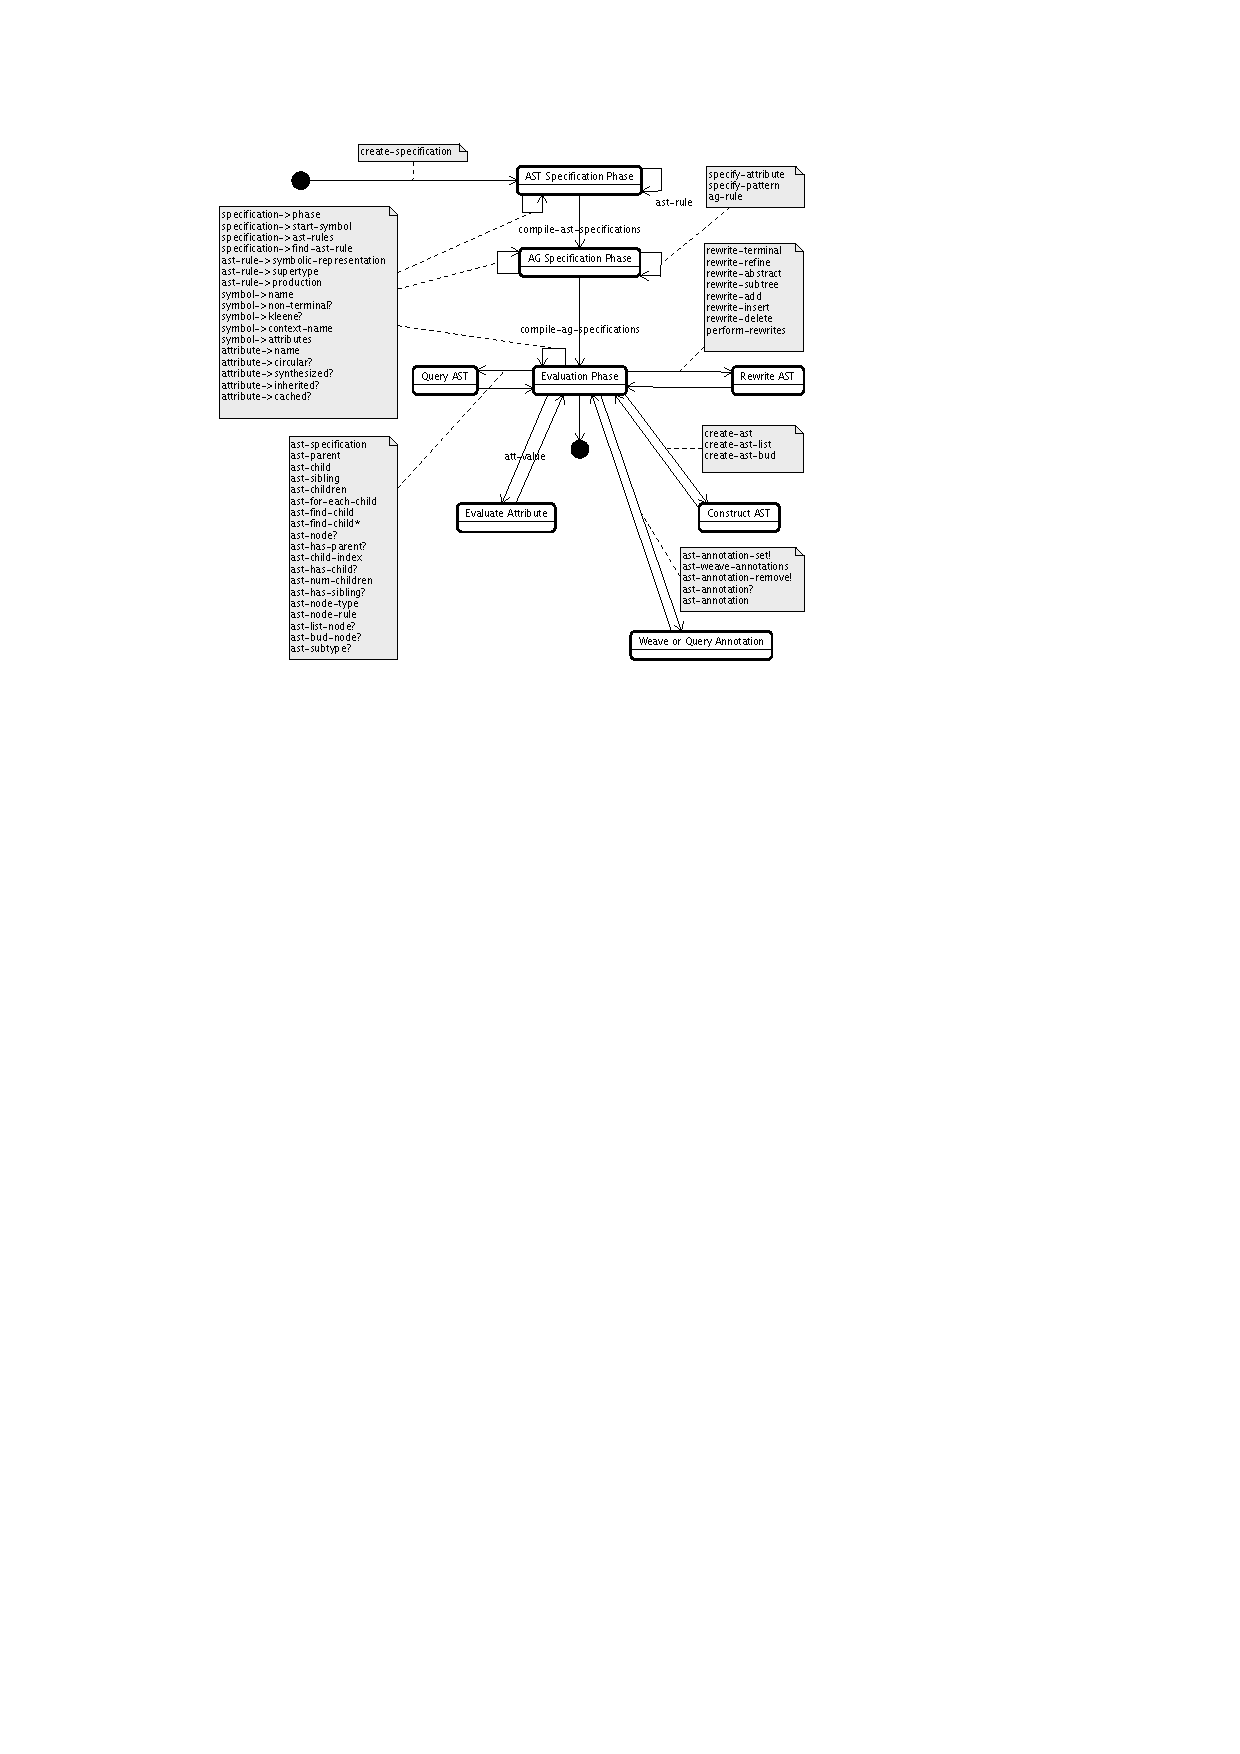
\includegraphics[width=0.9\linewidth]{../../documentation/figures/user-interface.pdf}
	\caption[Die RACR API]{RACR API~\cite{Buerger2012}}
	\label{fig:racr-api}
\end{figure}

%RACR macht sich zwei prägende Programmier-Paradigmen von Scheme zu eigen: RACR ist prozedural. Es existiert kein fester Zusammenhalt zwischen Daten und Funktionen, wie es bei der objektorientierten Programmierung der Fall ist. In der Scheme-Implementierung von RACR werden zur Speicherung der Spezifikationen und AST-Knoten bestimmte Scheme"=Records angelegt. RACR-spezifische Typen sind opak: Auf die einzelnen Felder dieser Records kann von außerhalb der RACR-Bibliothek nicht direkt zugegriffen werden. Ihr Aufbau widerspiegelt sich nicht in der Schnittstelle. Die wichtigsten RACR-spezifischen Datentypen sind \scm{racr-specification} und \scm{node}. RACR bietet Prozeduren, die diese Datenstrukturen zu erzeugen, und die auf sie angewandt werden können. Des Weiteren is RACR funktional. Einige Prozeduren RACRs erwarten eine Prozedur als Parameter. Dies betrifft vor allem die Attributsspezifikation.

\section{Das .NET-Framework und die Common Language Infrastructure}\label{sec:cli}

.NET ist ein von Microsoft entwickeltes Software-Framework und eine integrale Komponente des Windows-Betriebssystems. Für .NET entwickelte Programme werden nicht direkt nach Machinencode, sondern nach Bytecode – der Intermediate Language (IL) – übersetzt und laufen innerhalb eines virtuellen Ausführungssystems. Programmiersprachen, die nach IL kompilieren, werden .NET-Sprachen genannt, wobei C\# und Visual Basic .NET zu den wichtigsten Vertretern gehören. Der IL-Code wird in sogenannten Assemblies in Form von EXE-Dateien (Prozess-Assemblies) oder DLL-Dateien (Library-Assemblies) gespeichert.

Die stapelbasierende virtuelle Maschine (VM) von .NET wird innerhalb der Common Language Infrastructure (CLI)~\cite{ECMA2012}, einem internationalen Standard, definiert und bietet sprach-neutrale Features, wie zum Beispiel automatische Speicherbereinigung, Exceptions, Typsicherheit, Zugriff auf eine umfangreiche Klassenbibliothek und Just-in-Time-Kompilierung, wobei entsprechend der zu Grunde liegenden Rechnerarchitektur IL-Code bedarfsgesteuert zu nativem Code übersetzt wird. Neben der Common Language Runtime (CLR), der Microsoft-Implementierung der CLI, existieren Portable.NET\footnote{\url{http://www.dotgnu.org/}} und das Mono-Projekt\footnote{\url{http://www.mono-project.com/}} als kompatible, quelloffene Alternativen.

\begin{figure}
	\centering
	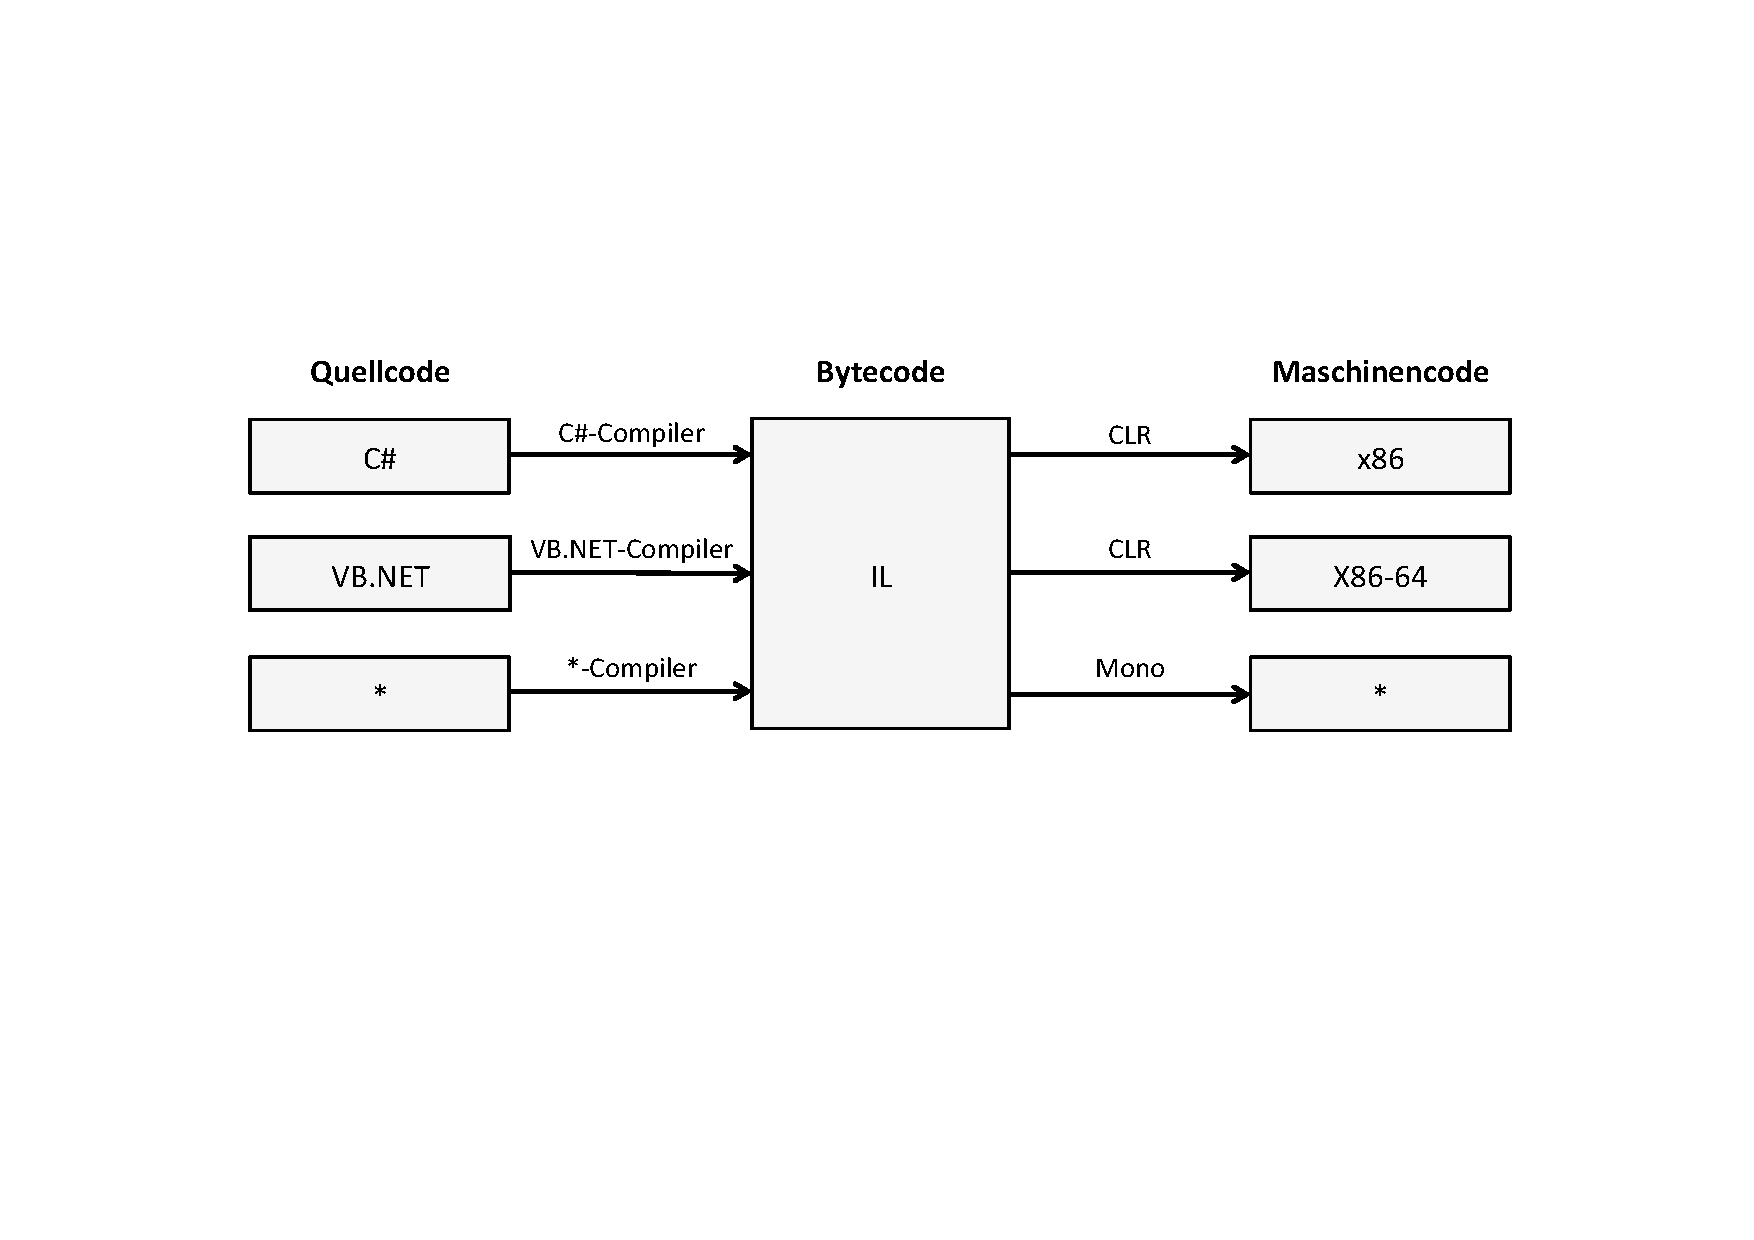
\includegraphics[width=0.9\linewidth]{figures/common-language-infrastructure.pdf}
	\caption{Übersetzung von .NET-Sprachen nach Maschinencode}
	\label{fig:cli}
\end{figure}

Abbildung~\ref{fig:cli} veranschaulicht die Kompillierungsprozesse, die der Ausführung eines .NET-Programms vorhergehen müssen. Alle .NET-Programme haben gleichen Bytecode, unabhängig von der Implementierungssprache oder der Zielarchitektur. Dies hat folgende wichtige Konsequenzen zur Folge:

\begin{itemize}
	\item .NET-Programme sind nicht architekturgebunden, sondern plattformunabhängig. Ein unter Windows entwickeltes Programm kann nach der Kompilierung unter Linux (mittels Mono) ausgeführt werden und umgekehrt.
	\item .NET-Sprachen haben zueinander hohe Interoperabilität. Die CLI vereinheitlicht unter anderem Exception-Handling, den Aufbau von und Zugriff auf Klassenbibliotheken und die Interaktion zwischen allen Datentypen. Objektinstanzen können über Sprachgrenzen hinweg ausgetauscht werden.
\end{itemize}

\section{IronScheme}

IronScheme\footnote{\url{http://ironscheme.codeplex.com/}} ist eine quelloffene, weitgehend R6RS-konforme Scheme-Implementierung für die .NET Software-Plattform. Sie umfasst einen eigenständigen, interaktiven Interpreter zur Ausführung von Scheme-Programmen und eine Klassenbibliothek, mittels welcher IronScheme in andere .NET-Projekte eingebunden werden kann. Diese Klassenbibliothek erlaubt es, .NET–Strings\footnote{Genauer gesagt handelt es sich um den Typ \csh{System.String} – die Klasse \csh{String} im Namensraum \csh{System}.} als Scheme-Ausdruck auszuwerten, analog zu der \scm{Eval}-Funktion, wie sie in vielen dynamischen Sprachen zu finden ist. So wird während der Programmausführung aus dem Scheme-Code IL-Code generiert und dieser anschließend ausgeführt. Scheme-Bibliotheken können jedoch auch zu Assemblies vorkompiliert werden.

\begin{table}[h!]
	\centering
	\begin{tabular}{@{}ll@{}}
		\toprule
			Scheme & .NET \\
		\midrule
			{\scm|fixnum|}		& {\csh|System.Int32|}			\\
			{\scm|flonum|}		& {\csh|System.Double|}			\\
			{\scm|boolean|}		& {\csh|System.Boolean|}		\\
			{\scm|string|}		& {\csh|System.String|}			\\
			{\scm|pair|}		& {\csh|IronScheme.Runtime.Cons|}	\\
			{\scm|'()|}		& {\csh|null|}				\\
			{\scm|hashtable|}	& {\csh|System.Collections.Hashtable|}	\\
			{\scm|symbol|}		& {\csh|Microsoft.Scripting.SymbolId|}	\\
			{\scm|procedure|}	& {\csh|Ironscheme.Runtime.Callable|}	\\
		\bottomrule		
	\end{tabular}
	\caption{IronSchemes Abbildung von Scheme-Datentypen auf .NET-Datentypen}
	\label{tab:typemapping}
\end{table}

Viele wichtige Datentypen sind als Adapter für .NET-Datentypen realisiert, was die Interoperabilität von IronScheme zu anderen .NET"=Sprachen erhöht. Andere Datentypen implementieren spezielle Schnittstellen. Die für diese Arbeit relevanten Scheme-Typen und deren zugehörige .NET-Typen sind in Tabelle~\ref{tab:typemapping} aufgeführt.

	% This program and the accompanying materials are made available under the
% terms of the MIT license (X11 license) which accompanies this distribution.

% Author: D. Langner, C. Bürger

\chapter{RACR-NET Implementierung: Prozedurale Schnittstelle}\label{umsetzung1}

Dieses Kapitel beschäftigt sich mit der Umsetzung einer prozeduralen Schnittstelle, welche es ermöglicht, RACR in C\# zu nutzen. Zuerst wird gezeigt, wie innerhalb von C\# Scheme-Code aufgerufen und wie die RACR-Scheme-Bibliothek effizient geladen werden kann. Nach einer Anforderungsanalyse wird die Implementierung vorgestellt. Die abschließende Evaluation zeigt die Schwächen einer rein prozeduralen Lösung und leitet zur finalen objektorientierten Lösung im folgenden Kapitel über.

\section{Scheme in C\#}

Mittels der IronScheme-Klassenbibliothek kann Scheme-Code von C\# aus ausgeführt werden. IronScheme bedient sich dazu der Extension-Methoden – ein Feature von C\#, das es erlauben, einem existierenden Typen neue Methoden hinzuzufügen, ohne den ursprünglichen Typ zu manipulieren. Extension-Methoden sind spezielle statische Methoden, die vom Nutzer wie Instanz-Methoden aufgerufen werden.

IronSchemes \csh{Eval} ist eine solche Methode. Sie interpretiert .NET-Strings als Scheme-Ausdrücke und gibt einen Wert vom Typ \csh{object} zurück, dem Basistypen aller .NET-Datentypen. Da C\# statisch typisiert ist, müssen Rückgabewerte zur sinnvollen Weiterverwendung üblicherweise explizit in einen Subtypen konvertiert werden. Deshalb bietet IronScheme auch eine generische Variante der \csh{Eval}-Methode. Diese akzeptiert einen Typ-Parameter, der den Typ des Rückgabewerts festlegt. Die Typumwandlung erfolgt hierbei innerhalb von \csh{Eval}.

Bei Referenztypkonvertierungen wie dieser kann während der Code-Übersetzung nicht bestimmt werden, ob die Umwandlung gültig ist. Schlägt zur Laufzeit eine Typumwandlungsoperation fehl, wird eine \csh{InvalidCastException} ausgelöst. Quelltext~\ref{csh:eval} veranschaulicht die Arbeitsweise von \csh{Eval}.

\begin{lstlisting}[language=csh, caption={Auswerten von Scheme-Ausdrücken}, label=csh:eval]
object a = "(+ 1 2)".Eval();
int b = (int) a;					// explizite Umwandlung
bool c = "(< 3 4)".Eval<bool>();	// generische Methode

bool d = (bool) "(* 2 3)".Eval();	// Laufzeitfehler!
bool e = "(* 2 3)".Eval<bool>();	// Laufzeitfehler!
\end{lstlisting}

Alle Scheme-Prozeduren implementieren das \csh{Callable}"=Interface, mittels welchem man eine Prozedur ohne mehrfaches Parsen oder Kompilieren wiederholt aufrufen kann. Diese abstrakte Klasse stellt \csh{Call}"=Methoden in verschiedenen Ausführungen bereit – variierend über die Anzahl von Parametern, welche wie auch der Rückgabewert stets vom Typ \csh{object} sind. Auf diese Weise wird die dynamische Typisierung von Scheme in C\# abgebildet. Beim Aufruf eines \csh{Callable}"=Objektes kann der Compiler für die korrekte Stelligkeit sowie die Typisierung der Parameter einer Prozedur nicht garantieren. Typfehler äußern sich erst während der Laufzeit eines Programms. Quelltext~\ref{csh:call} zeigt das Interface in Aktion.

\begin{lstlisting}[language=csh, caption={Verwendung des \csh{Callable}"=Interfaces}, label=csh:call]
Callable sum = "+".Eval<Callable>();
int a = (int) sum.Call(1, 2);
int b = (int) sum.Call(3, 4, 5);
int c = (int) sum.Call(0, false);	// Laufzeitfehler!
\end{lstlisting}

\section{RACR in C\#}

\subsection{Importieren der Scheme-Bibliothek}

Der nächste Schritt besteht darin, RACR dem Scheme-Environment bekannt zu machen. RACR laden wir mittels \csh{"(import (racr core))".Eval()}. Dieser Aufruf veranlasst IronScheme dazu, den Quellcode RACRs, der in der Datei \verb|racr/core.sls| residiert, zu kompilieren und alle darin als Export deklarierten Symbole zu registrieren. Dies geschieht mit jedem Neustart des C\#-Programms, was dessen Anlaufzeit verlängert.

Ein weniger dokumentiertes Feature IronSchemes erlaubt es, Scheme-Bibliotheken vorzukompilieren und in Assemblies zu speichern. Auf diese Weise kann das Laden von RACR stark beschleunigt werden. Zum Beispiel lege man eine Datei namens \verb|tmp.scm| mit dem Inhalt \scm{(import (racr core))} an. Der Aufruf von \scm{(compile "tmp.scm")} in der interaktiven IronScheme"=Konsole generiert die Datei \verb|racr.core.dll|. Wenn diese Assembly bei der Kompilierung eines C\#"=Programms referenziert wird, so kompiliert IronScheme RACR mit dem Aufruf von \scm{import} nicht neu, sondern lädt den kompilierten Code aus der DLL"=Datei.

\subsection{Konformitätsprüfung von IronScheme}

Wie im vorhergehenden Kapitel beschrieben, unterscheiden sich Scheme-Interpreter bezüglich ihrer R6RS-Konformität. Um die korrekte Funktion von RACR unter Verwendung verschiedener Interpreter zu gewährleisten, beinhaltet RACR eine Test-Umgebung, die dessen wesentlichen Funktionsumfang abdeckt. Diese Tests wurden mit IronScheme ausgeführt. Dabei terminierten vorerst alle Tests mit dem gleichen Fehler: Der Aufruf von \scm{hashtable-set!} mit dem Schlüssel \scm{'()} löst eine \csh{System.ArgumentNullException} aus. Der Fehler wird durch eine R6RS-Unkonformität IronSchemes verursacht: RACR benutzt häufig die leere Liste als Schlüssel, um Daten in einer \scm{hashtable}"=Datenstruktur abzulegen. Wie Tabelle~\ref{tab:typemapping} zu entnehmen, bildet IronScheme \scm{hashtable} auf den CLI-internen Typ \csh{System.Collections.Hashtable} ab. Des Weiteren wird die leere Liste \scm{'()} auf \csh{null} abgebildet. Laut MSDN\footnote{ \url{https://msdn.microsoft.com/library/system.collections.hashtable.aspx}} darf der Schlüssel eines \csh{Hashtable}"=Objektes jedoch nicht \csh{null} sein.

Ein Workaround in Form einer Scheme-Bibliothek soll bijektiv die leere Liste auf einen internen Record abbilden. Quelltext~\ref{scm:hash} zeigt die Definition dieses Records und dessen Verwendung in den Prozeduren \scm{hashtable-ref*} und \scm{hashtable-set!*}, welche das Interface von \scm{hashtable-ref} beziehungsweise \scm{hashtable-set!} reimplementieren.

\begin{lstlisting}[language=scm, caption={\scm{hashtable}"=Workaround}, label=scm:hash]
(define-record-type nil-record (sealed #t) (opaque #t))
(define nil (make-nil-record))

(define hashtable-ref*
  (lambda (h key default-value)
    (hashtable-ref h (if (null? key) nil key) default-value)))

(define hashtable-set!*
  (lambda (h key value)
    (hashtable-set! h (if (null? key) nil key) value)))
\end{lstlisting}

Auf Zeile~1 wird ein neuer Record-Typ angelegt und anschließend auf Zeile~2 instanziiert. In den Definitionen der \scm{hashtable}"=Prozeduren wird mittels einer \scm{if}"=Anweisung geprüft, ob es sich bei dem Schlüssel um das \scm{null}"=Objekt handelt, in welchem Falle der \scm{nil}"=Record als Schlüssel benutzt werden soll (Zeilen~6 und 10). Auf ähnliche Weise wurde das Interface folgender weiterer Scheme-Prozeduren reimplementiert: \scm{hashtable-delete!}, \scm{hashtable-contains?} und \scm{hashtable-entries}. Diese Bibliothek wurde in RACR eingebunden und alle Aufrufe der genannten Prozeduren auf die entsprechenden Reimplementierungen umgelenkt. Alle Tests der RACR"=Test-Umgebung liefen nun fehlerlos. Somit ist sichergestellt, dass RACR unter IronScheme korrekt ausgeführt wird.

\section{Anforderungsanalyse}\label{anforderungen1}

Um die Qualität der RACR"=C\#"=Schnittstelle bewerten zu können, müssen geeignete Kriterien festgelegt werden. Bislang steht dem Programmierer RACR nur als Scheme-Bibliothek zur Verfügung. Folglich müssen sämtliche Aspekte einer Anwendung, die den Funktionsumfang von RACR nutzen sollen, in Scheme programmiert sein. Mit der Möglichkeit, RACR auch in C\# nutzen zu können, ergeben sich neue Anwendungsfälle, in denen die verschiedenen Aspekte einer RACR-Anwendung zu variierenden Anteilen in Scheme oder C\# implementiert sein können. In einem Beispiel-Szenario werden AST"=Regeln und Attribute einer Sprachspezifikation in Scheme definiert. Mittels dieser Spezifikation werden von C\# aus ASTs instanziiert und Analysen betrieben. Ein weiterer denkbarer Fall ist, dass eine in Scheme spezifizierte Sprache in C\# um zusätzliche Attribute erweitert wird. Abbildung~\ref{fig:usecase} visualisiert diese und weitere Szenarien. Es ergibt sich eine Vielzahl möglicher Varianten der Sprachnutzung, Kopplung und Vererbung und der Aufteilung deren Implementierungen in Scheme und C\#.

Diese Arbeit fokussiert sich auf das Szenario, in dem der Nutzer RACR ausschließlich von C\# aus bedient. Angesichts dessen werden folgende Anforderungen an das System gestellt:

\begin{figure}
	\centering
	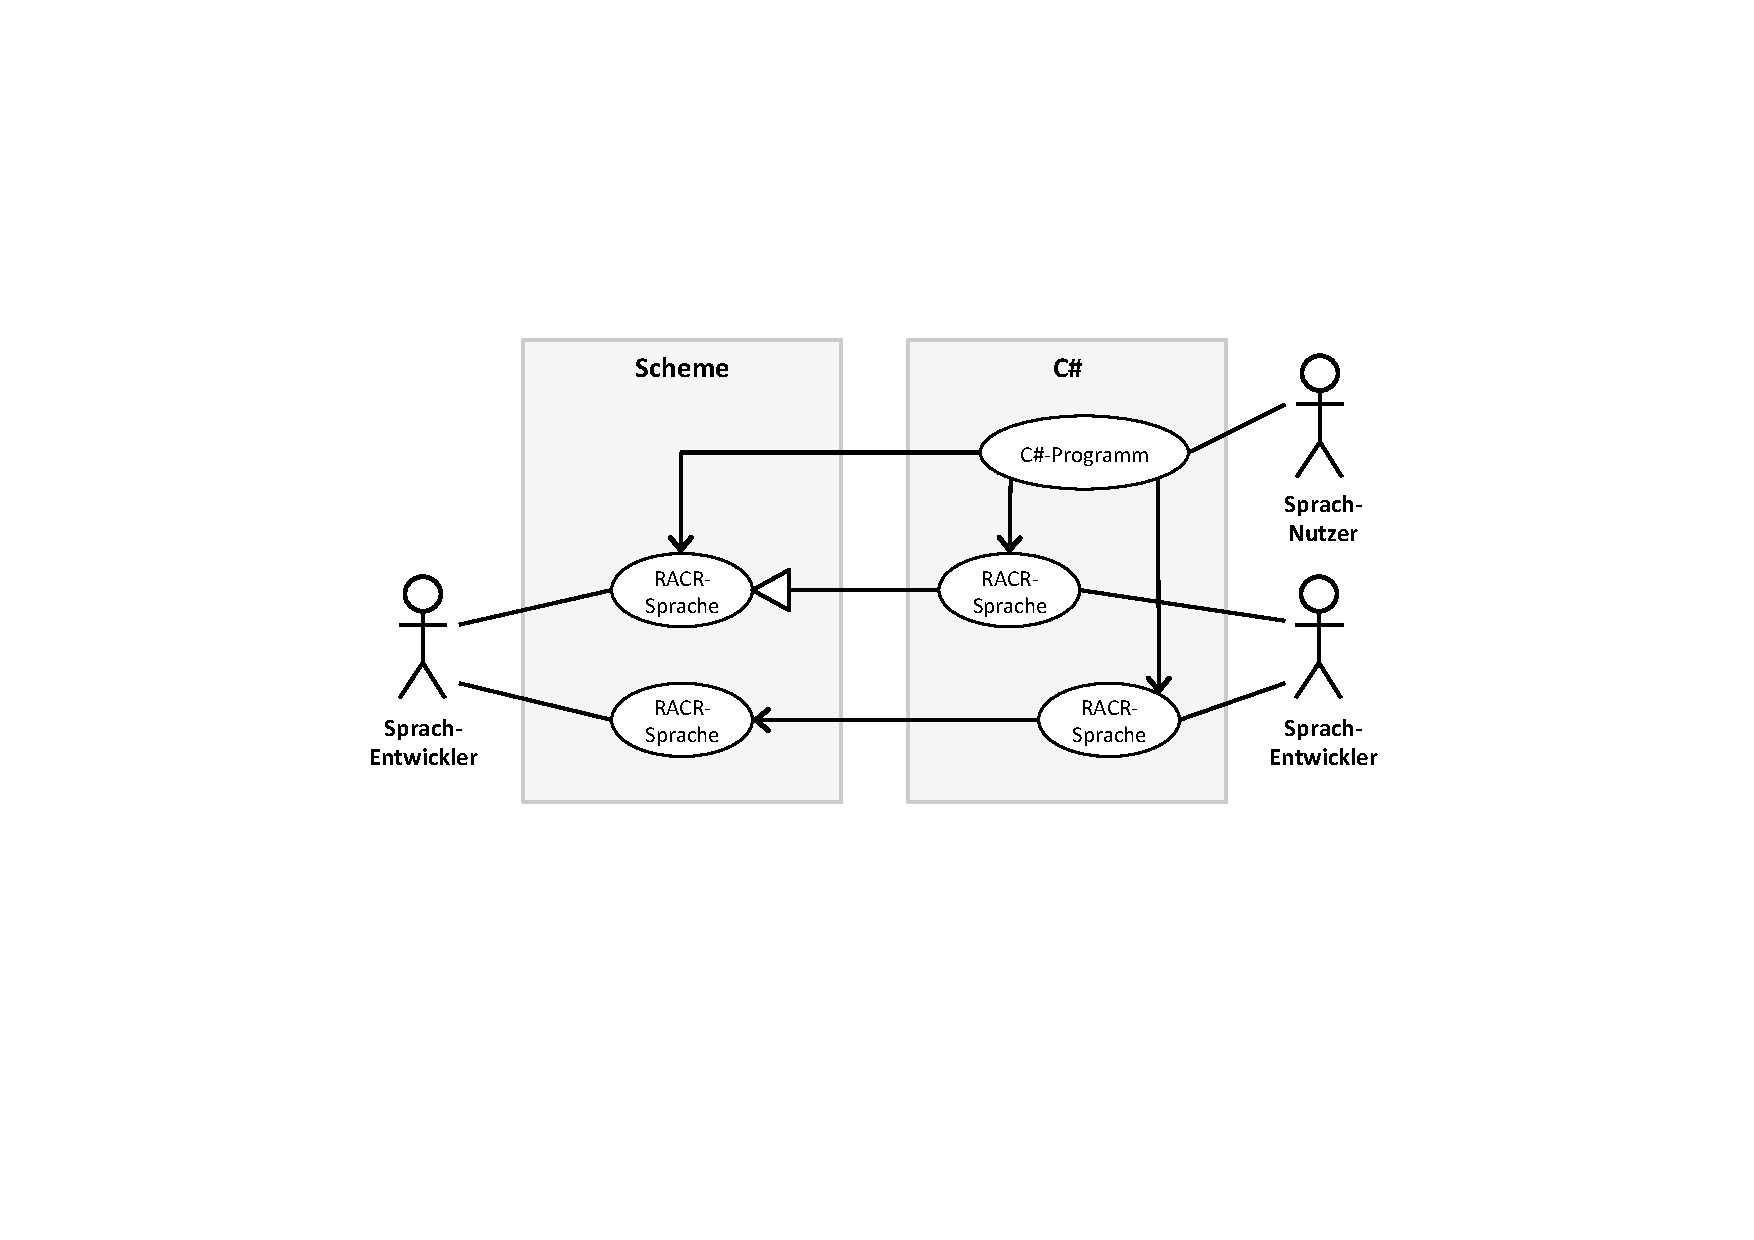
\includegraphics[width=0.9\linewidth]{figures/racr-net-use-cases.pdf}
	\caption{Anwendungsfälle von RACR in Scheme und C\#}
	\label{fig:usecase}
\end{figure}

\begin{description}
	\item[A1 – Vollständigkeit:] Alle dokumentierten~\cite{Buerger2012} Funktionalitäten, die RACR in Scheme bietet, sollen uneingeschränkt auch von C\# aus nutzbar sein.
	\item[A2 – Dynamik:] Die dynamische Natur RACRs muss erhalten bleiben. Grammatik und Attribute sollen noch während der Programmlaufzeit festgelegt werden können. Dies schließt Code-Generatoren, die anhand einer Spezifikation C\#-Code erzeugen, aus.
	\item[A3 – Nähe zur originalen Schnittstelle:] Der Wechsel zwischen Scheme und C\# soll für mit RACR vertraute Programmierer intuitiv sein.
	\item[A4 – Entkoppelung von Scheme:] Dass im Hintergrund die eigentliche Arbeit in einer Scheme-VM passiert, soll für C\#"=Nutzer irrelevant sein und sich in keinster Weise in der Schnittstelle widerspiegeln. Insbesondere sollen IronScheme"=eigene Datentypen, wie zum Beispiel Paare, nicht in der Schnittstelle vorkommen. Stattdessen sollen äquivalente, .NET-typische Typen zum Einsatz kommen.
\end{description}

Im Nachfolgenden soll eine funktionierende, zunächst prozedurale Schnittstelle geschaffen werden, welche die Anforderungen \textbf{A1} bis \textbf{A4} erfüllt. Die endgültige objektorientierte Schnittstelle wird in Kapitel~\ref{umsetzung2} behandelt.

\section{Implementierung der prozeduralen Schnittstelle}

Die prozedurale Schnittstelle soll vollständig sein und die Funktionsweise RACRs nicht einschränken. Ein naiver Ansatz zur Implementierung einer solchen Schnittstelle besteht darin, für jede Scheme-Prozedur in C\# ein direktes Gegenstück zu modellieren – in Form einer statischen Methode. Innerhalb dieser Methoden soll unter Verwendung der IronScheme-VM die entsprechende Prozedur aufgerufen werden. Auf diese Weise werden die Anforderungen \textbf{A1} und \textbf{A2} erfüllt.

Um Anforderung \textbf{A3} zu befriedigen, müssen die Methodennamen denen der zugehörigen Prozeduren gleichen. RACR hält sich bei der Benennung von Variablen beziehungsweise Prozeduren an die für Lisp-Sprachen typischen Konventionen und verwendet in Bezeichnern einige Sonderzeichen. Beispielsweise werden innerhalb eines Bezeichners Worte durch Bindestriche getrennt. Bezeichner von Prozeduren, die einen booleschen Wert liefern, enden für gewöhnlich mit einem Fragezeichen. C\# hat seine eigenen Namenskonventionen. Sonderzeichen in Bezeichnern sind nicht gestattet. Alle Namen öffentlicher Member, Typen und Namespaces beginnen mit einem Großbuchstaben, Parameternamen jedoch mit einem Kleinbuchstaben. Beiderseits werden innerhalb eines Bezeichners verkettete Wörter durch Binnenmajuskel hervorgehoben.

Bei der Benennung der Methoden der .NET-Schnittstelle für RACR soll die C\#-übliche Namenskonvention eingehalten werden ohne den Prozedurnamen zu entfremden. Aus \scm{create-ast} wird \csh{CreateAst}. Alle anderen Benennungen geschehen analog. Somit wird die Realisierung von Anforderung \textbf{A3} gewährleistet. Quelltext~\ref{csh:naiv} skizziert diesen Ansatz.

\begin{lstlisting}[language=csh, caption={Prozedurale C\#"=Schnittstelle für RACR}, label=csh:naiv]
public static class Racr {
	private static Callable createSpecification;
	private static Callable astRule;
	// ...
	static Racr() {
		"(import (racr core))".Eval();
		createSpecification	= "create-specification".Eval<Callable>();
		astRule				= "ast-rule".Eval<Callable>();
		// ...
	}
	public static object CreateSpecification() {
		return createSpecification.Call();
	}
	public static void AstRule(object spec, string rule) {
		astRule.Call(spec, SymbolTable.StringToObject(rule));
	}
// ...
\end{lstlisting}

Die statische Klasse \csh{Racr} umfasst private \csh{Callable}"=Felder, die Referenzen auf die entsprechenden Scheme-Prozeduren RACRs speichern sollen. Im statischen Konstruktor wird zuerst die RACR"=Bibliothek geladen (Zeile~6), woraufhin alle \csh{Callable}"=Objekte initialisiert werden. Zusätzlich enthält die Klasse für jedes \csh{Callable} eine statisch Methode, die als Adapter fungiert, indem sie ihre Argumente an die \csh{Call}"=Methode des entsprechenden \csh{Callable}"=Objekt durchreicht und dessen Rückgabewert zurückliefert. Ein triviales Beispiel hierfür ist die parameterlose Methode \csh{CreateSpecification} (Zeile~11).

\subsection{Entkopplung von Scheme}

Um die Anforderung \textbf{A4} zu erfüllen, werden gegebenenfalls Umwandlungen Scheme-eigener Datentypen erforderlich. RACR nutzt Symbole, Paare und Listen – sowohl für Funktionsparameter als auch für Rückgabewerte. Des Weiteren erwarten einige Prozeduren als Argument selbst eine Prozedur. Der Umgang mit diesen Scheme-typischen Datentypen von C\# aus ist unbequem und ineffizient, weswegen sie in RACRs C\#"=Schnittstelle vermieden werden sollen, sodass der Nutzer nicht mit ihnen konfrontiert wird. An ihrer statt sollen charakteristischere Typen zum Einsatz kommen. Die Implementierung der Schnittstelle muss für die Übersetzung solcher Typen Sorge tragen. Im Folgenden soll auf jene Datentypen eingegangen werden, die zur Verarbeitung in C\# einer Sonderbehandlung bedürfen.

\subsubsection{Symbole}

Scheme-Symbole tauchen in RACRs Schnittstelle an vielen Stellen auf. Aufseiten von C\# sollen stattdessen .NET-Strings zum Einsatz kommen. Symbole werden unter anderem als Zeichenketten für Nichtterminale, ganze AST-Regeln und Attributsnamen verwendet. IronScheme implementiert Symbole mittels der Struktur \csh{SymbolId}, deren \csh{ToString} Methode die String-Repräsentation der jeweiligen Symbol-Instanz liefert. Analog bildet die statische Methode \csh{SymbolTable.StringToObject} Strings auf Symbole ab. Quelltext~\ref{csh:naiv} zeigt die Verwendung von \csh{SymbolTable.StringToObject} in der Methode \csh{AstRule} (Zeile~15).

\subsubsection{Paare}

Paare sind in Scheme ein essenzieller Datentyp. In RACRs Scheme"=Schnittstelle kommen Paare in folgenden Prozeduren zum Einsatz: \scm{ast-children}, \scm{ast-for-each-child}, \scm{ast-find-child} und \scm{ast-find-child*}. Diese Prozeduren verlangen neben anderen Arguenten eine unbestimmte Anzahl von sogenannten Kinder-Intervallen – Paare, die in Form von zwei Indices eine untere und ober Grenze enthalten. Mit dem Scheme-Symbol \scm{'*} kann auch eine offene obere Grenze angegeben werden\footnote{\url{https://github.com/christoff-buerger/racr/blob/master/documentation/abstract-syntax-trees.md\#ast-children}}. Paare entsprechen in C\# Objekten der Klasse \csh{Cons} aus der IronScheme-Klassenbibliothek. Nutzer sollen mit ihr nicht in Berührung kommen müssen, sondern zur Angaben von Kinder-Intervallen eine für genau diesen Zweck geschaffene Datenstruktur verwenden. Quelltext~\ref{csh:range} zeigt die dafür konzipierte Struktur \csh{Range}.

\begin{lstlisting}[language=csh, caption={Definition der \csh{Range}"=Struktur}, label=csh:range]
public struct Range {
	public int min;
	public int max;
	public Range(int min, int max=0) {
		this.min = min;
		this.max = max;
	}
	internal Cons ToCons() {
		return new Cons(min,
						max > 0 ? max : SymbolTable.StringToObject("*"));
	}
}
\end{lstlisting}

Zweckmäßig hält die Struktur zwei Felder für die beiden Grenzen, wobei eine obere Grenze mit dem Wert 0 als offen interpretiert wird\footnote{In RACR werden Indices stets von 1 an gezählt.}. Die interne Methode \csh{ToCons} dient dazu, aus dem \csh{Range}"= ein \csh{Cons}"=Objekt zu konstruieren, das von IronScheme aus weiterverarbeitet werden kann. Sie kommt in den Methoden des Interfaces, welche die oben genannten Prozeduren abbilden sollen, zum Einsatz.

\subsubsection{Listen}

Scheme-Listen sind verschachtelte Scheme-Paare. Sie sind ein Parameter der Prozeduren \scm{create-ast} und \scm{create-ast-list} und der Rückgabetyp der Prozeduren \scm{ast-children} und \scm{rewrite-abstract}. Analog zu \scm{create-ast-list}, erwartet die \scm{create-ast} als letztes Argument eine Liste mit den Kindern des zu erzeugenden AST-Knoten. In der C\#"=Schnittstelle soll für den Nutzer der Zwischenschritt, erst eine Liste für die Kinder zu konstruieren, übersprungen werden. Stattdessen soll die Methode \csh{CreateAst} ein C\#"=Array von Kind-Knoten akzeptieren. Unter Verwendung einer einfachen Schleife über das Array soll daraus die Scheme-Liste erzeugt werden, damit sie anschließend beim Aufruf der Scheme-Prozedur übergeben werden kann.

\begin{lstlisting}[language=csh, caption={Listenkonstruktion in \csh{CreateAst}}, label=csh:createast]
public static object CreateAst(object spec, string nonTerm,
							   params object[] children)
{
	Cons list = null;
	for (int i = children.Length - 1; i >= 0 ; i--) {
		list = new Cons(children[i], list);
	}
	return createAst.Call(spec, SymbolTable.StringToObject(nonTerm),
						  list);
}

\end{lstlisting}

Quelltext~\ref{csh:createast} zeigt die Implementierung der Methode \csh{CreateAst} der Klasse \csh{Racr} gemäß den oben genannten Vorgaben. Man beachte, dass dem Parameter \csh{children} das Schlüsselwort \csh{params} vorangestellt ist. Es bewirkt, dass beim Aufruf der Methode eine variable Anzahl von Methodenargumenten automatisch zu einem Array zusammengefasst wird, sodass der Nutzer das Array nicht selbst anzulegen braucht. Will man beispielsweise einen Knoten mit drei Kind-Knoten erzeugen, gestaltet sich der Aufruf von \csh{CreateAst} wie folgt:

\begin{lstlisting}[language=csh, numbers=none]
object node = Racr.CreateAst(spec, "A", childA, childB, childC);
\end{lstlisting}

Auch als Rückgabewert sollen in der C\#"=Schnittstelle Scheme-Listen durch Arrays ersetzt werden. Die in Quelltext~\ref{csh:rewriteabstract} abgebildete Implementierung von \scm{RewriteAbstract} nutzt eine \csh{while}"=Schleife, um die Kette von \csh{Cons}"=Objekten zu durchwandern und die in der Liste gespeicherten Kind-Knoten einer \csh{List<object>} anzuhängen. Die Klasse \csh{List} ist Teil der .NET-Klassenbibliothek. Im Gegensatz zum Array bietet sie Methoden, um die Anzahl ihrer Elemente dynamisch zu ändern.

\begin{lstlisting}[language=csh, caption={Arraykonstruktion in \csh{RewriteAbstract}}, label=csh:rewriteabstract]
public object[] RewriteAbstract(string supertype) {
	var list = rewriteAbstract.Call(ast,
			   SymbolTable.StringToObject(supertype)) as Cons;
	var children = new List<object>();
	while (list != null) {
		children.Add(list.car);
		list = list.cdr as Cons;
	}
	return children.ToArray();
}
\end{lstlisting}

\subsubsection{Prozeduren}\label{prozeduren}

Schemes Prozeduren sind First-Class-Objekte und können Funktionen als Argumente überreicht werden. Insofern ist Scheme eine höhere, funktionale Sprache. Wie schon erwähnt, sind Prozeduren aus der Sicht von .NET Subtypen der abstrakten Klasse \csh{Callable}. C\# unterstützt First-Class-Funktionen in Form von Delegaten – Referenztypen, mit denen eine benannte oder anonyme Methode gekapselt werden kann. Sie haben Ähnlichkeit mit Funktionszeigern in C. Der Typ eines Delegat-Objektes entspricht einer bestimmten Methodensignatur, die sich aus der Anzahl und den Typen der Parameter und dem Rückgabetyp zusammensetzt. Um C\#"=Methoden an RACR zu übergeben, müssen diese zuerst in ein \csh{Callable} umgewandelt werden. IronScheme bietet zu diesem Zweck die Extension-Methode \csh{ToSchemeProcedure} der Klasse \csh{Delegate}, die Basisklasse aller Delegat-Typen. Innerhalb von RACR erwarten folgende Prozeduren eine Funktion als Argument: \scm{ast-for-each-child}, \scm{ast-find-child}, \scm{ast-find-child*} und \scm{specify-attribute}. Dabei gleichen sich die ersten drei insofern, dass die Signatur der zu übergebenden Prozedur von RACR vorgegeben ist, woraus sich für die C\#"=Schnittstelle ein entsprechender Delegat-Typ ergibt.

\begin{lstlisting}[language=csh, caption={Delegat-Parameter in \csh{AstFindChild}}, label=csh:astfindchild]
public static object AstFindChild(object node, Func<int,object,bool> f,
								  params Range[] bs)
{
	object[] args = new object[2 + bs.Length];
	args[0] = f.ToSchemeProcedure();
	args[1] = node;
	for (int i = 0; i < bs.Length; i++) args[i + 2] = bs[i].ToCons();
	object res = astFindChild.Call(args);
	if (res is bool && (bool) res == false) return null;
	return res;
}
\end{lstlisting}

Quelltext~\ref{csh:astfindchild} zeigt die Implementierung von \csh{AstFindChild}. Die Methode ist variadisch, genau wie die Scheme-Prozedur, an die sie ihre Argumente weiterleiten muss. Um eine unbestimmte Anzahl von Argumenten an den Aufruf eines \csh{Callable}"=Objekts weiterzugeben, müssen diese in ein Objekt-Array geschrieben werden, welches als einziger Parameter an \csh{Call} übergeben werden muss. Zeile~4 deklariert dieses Array und die drei darauffolgenden Zeilen befüllen es. Dem Delegat-Typen \csh{Func<int,object,bool>} zufolge muss die zu übergebende Funktion zwei Parameter mit den Typen \csh{int} und \csh{object} für den Index des Knoten beziehungsweise den Knoten selbst habe, nebst dem Rückgabetypen \csh{bool}. \csh{ToSchemeProcedure} nutzt die durch Introspektion zugänglichen Typinformationen, um ein \csh{Callable}"=Objekt zu generieren, in welchem der Delegat gekapselt wird. Die Methode \csh{AstFindChild} weicht in ihrem Verhalten von \scm{ast-find-child} ab, indem sie bei einer missglückten Suche statt \csh{false} \csh{null} zurückgibt (Zeile~9). Dies entspricht der in C\# üblichen Weise, das Fehlen eines Objektes zu kennzeichnen.

Der Aufruf von \csh{AstFindChild} gestaltet sich unter Benutzung von C\#'s Lambda-Ausdrücken elegant. Hier ein Beispiel:

\begin{lstlisting}[language=csh]
object child = Racr.AstFindChild(parent, (i, n) => {
		bool success;
		// setze success anhand von Attributsauswertungen, etc.
		return success;
	}, new Racr.Range(2, 7));
\end{lstlisting}

Mit \scm{specify-attribute} lassen sich (gegebenenfalls Referenz-) Attribute definieren. Dieser Prozedur muss dabei unter anderem eine Attributgleichung (in Form eines Delegaten) übergeben werden. RACR unterstützt parametrisierte Attribute, was sich darin äußert, dass die Attributgleichungsfunktion neben einem Argument für den AST-Knoten noch weitere Argumente akzeptiert, mit welchem die auszuwertende Instanz des Attributes assoziiert ist. Bei der Attributsauswertung mittels \scm{att-value} muss die entsprechende Anzahl an Argumenten des Attributs mit übergeben werden. Für die Korrektheit der Argumenttypen ist stets der Programmierer allein verantwortlich.

Aus der Sicht einer statisch typisierten Sprache wie C\# stellt diese Dynamik in der Attributsspezifikation und -auswertung eine Herausforderung dar, da der exakte Typ der Attributgleichungsfunktion beinahe beliebig sein kann: Nur der erste Parameter wird von RACR als AST-Knote vorgegeben. Die Implementierung der Methodengruppe \csh{SpecifyAttribute}\footnote{Der Einfachheit halber ist hier eine Implementierung gezeigt, die keine zyklischen Attribute unterstützt.} ist in Quelltext~\ref{csh:specifyattribute} abgebildet. Die erste Methode besitzt für die Attributgleichung einen Parameter vom Typ \csh{Delegate}. Lambda-Ausdrücke werden vom Compiler jedoch nicht implizit nach \csh{Delegate} umgewandelt. Um den Nutzer dennoch von verbosen Typumwandlungen zu entlasten, decken die zwei zusätzlichen generischen Ausführungen von \csh{SpecifyAttribute} den Fall für parameterlose (\csh{Func<object,R>}) beziehungsweise mit einem Parameter parametrisierte (\csh{Func<object,T,R>}) Attribute ab.

\begin{lstlisting}[language=csh, caption={Methodengruppe \csh{SpecifyAttribute}}, label=csh:specifyattribute]
public static void SpecifyAttribute(object spec, string name,
		string nonTerm, string context, bool cached, Delegate eq)
{
	specifyAttribute.Call(spec,
						  SymbolTable.StringToObject(name),
						  SymbolTable.StringToObject(nonTerm),
						  SymbolTable.StringToObject(context),
						  cached,
						  eq.ToSchemeProcedure(),
						  false);
}
public static void SpecifyAttribute<R>(object spec, string name,
		string nonTerm, string context, bool cached, Func<object,R> eq)
{
	SpecifyAttribute(spec, name, nonTerm, context, cached, (Delegate) eq);
}
public static void SpecifyAttribute<T,R>(object spec, string name,
		string nonTerm,	string context, bool cached, Func<object,T,R> eq)
{
	SpecifyAttribute(spec, name, nonTerm, context, cached, (Delegate) eq);
}
\end{lstlisting}

Um den Einsatz von \csh{SpecifyAttribute} vorzuführen, definiert folgender C\#"=Code das parameterlose Attribut \verb|value| für den Knotentypen \verb|Addition|:

\begin{lstlisting}[language=csh]
Racr.SpecifyAttribute(spec, "Eval", "Addition", "*", true, (n) => {
	return (int) Racr.AttValue(Racr.AstChild(n, 1), "value")
		 + (int) Racr.AttValue(Racr.AstChild(n, 2), "value");
});
\end{lstlisting}

Dies entspricht folgender Attributspezifikation in Scheme:

\begin{lstlisting}[language=scm]
(with-specification spec
  (ag-rule
    value
    (Addition
      (lambda (n)
        (+ (att-value 'value (ast-child 1 n))
           (att-value 'value (ast-child 2 n)))))))
\end{lstlisting}

\subsection{Evaluation der Schnittstelle}\label{evaluation1}

Die resultierende Schnittstelle deckt den vollständigen Funktionsumfang RACRs ab (\textbf{A1}). Sprachspezifikationen können zur Programmlaufzeit dynamisch definiert werden (\textbf{A2}). Obschon die Schnittstelle sehr dem Original ähnelt (\textbf{A3}), wird der Nutzer zu keiner Zeit mit konkreten Scheme-Typen konfrontiert (\textbf{A4}).

Die Schnittstelle hat jedoch zwei entscheidende Schwächen: Für Sprachspezifikationen und AST-Knoten fehlen konkrete Typen. Die entsprechenden RACR-spezifischen Objekttypen, auf denen alle RACR-Prozeduren arbeiten, sind Scheme-Records mit den Namen \scm{ast-specification} beziehungsweise \scm{node}. Diese Datentypen werden erst zur Programmlaufzeit generiert. IronScheme kann für Instanzen solcher Typen keinen präziseren Subtypen als \csh{object} geben. Effektiv handelt es sich hierbei um opake Handler, ähnliche den \csh{void}–Zeigern in C. Deshalb sind Spezifikationen sowie AST-Knoten in der Schnittstelle stets als \csh{object} typisiert. Konsequenterweise ist aus der Signatur einer RACR-Methode allein nicht klar ersichtlich, welcher tatsächliche Objekttyp erwartet wird, was eine Quelle von Typfehlern darstellt, die während der Übersetzung nicht erkannt werden können.

Eine weitere Schwachstelle besteht in der Benutzerfreundlichkeit der Schnittstelle, die dem Nutzer einen prozeduralen Programmierstil aufdrängt. Objektorientierung, die Grundcharakteristik von C\#, wird nicht wirkungsvoll eingesetzt.

Aus den vorgestellten Nachteilen ergeben sich die folgenden zusätzlichen Anforderungen an die bereits in Kapitel~\ref{anforderungen1} präsentierten:

\begin{description}
	\item[A5 – Entkoppelung von der RACR-Implementierung:] Der Nutzer soll nicht direkt mit den Handlern für \scm{ast-specification} und \scm{node} arbeiten. Opake RACR-Datentypen sollen in Stellvertreter-Objekten gekapselt werden.	
	\item[A6 – Objektorientierung:] Alle wesentlichen Prozeduren von RACR können entweder Spezifikationen oder AST-Knoten zugeordnet werden. Die C\#"=Schnittstelle soll diese Prozeduren als Methoden der entsprechenden Objekte bereitstellen.
\end{description}

	% This program and the accompanying materials are made available under the
% terms of the MIT license (X11 license) which accompanies this distribution.

% Author: D. Langner, C. Bürger

\chapter{RACR-NET Implementierung: Objektorientierte Schnittstelle}\label{umsetzung2}

Dieses Kapitel beschäftigt sich mit der Verwirklichung einer objektorientierten C\#"=Schnittstelle für RACR: RACR-NET\footnote{Die Quellen von RACR-NET sind bereits in denen von RACR aufgenommen und stehen unter MIT-Lizenz zur Verfügung.}. Dabei sollen die in Kapitel~\ref{evaluation1} für verbesserungswürdig befundenen Probleme der prozeduralen Schnittstelle gelöst werden. Erreicht wird dies durch Refactoring der prozeduralen Schnittstelle. Die Idee hierbei ist, dass dessen Funktionalitäten entweder für RACR-Spezifikationen oder AST-Knoten definiert sind, sich also in zwei entsprechende Klassen partitionieren lassen (\csh{RACR.Specification} und \csh{RACR.AstNode}). Jede statische Methode der prozeduralen Schnittstelle (außer dem statischen \csh{Racr}"=Konstruktor) wird in eine Objektmethode einer der beiden Klassen umgeformt.

Die folgenden Unterkapitel stellen zunächst die resultierende objektorientierte Schnittstelle vor und demonstrieren deren Verwendung anhand eines Beispiels. Danach wird auf Details der Implementierung eingegangen. Eine Evaluation der Schnittstelle erfolgt in Kapitel~\ref{ausblick}.

\section{Überblick über die objektorientierte Schittstelle}

Im Folgenden wird lediglich die Schnittstelle für Sprachspezifikationen und AST-Knoten eingeführt. Auf konkrete Details ihrer Implementierung wird in Kapitel~\ref{implementierung} eingegangen.

\subsection{Spezifikationsschnittstelle}\label{spezifikation}

\csh{RACR.Specification} ist die Hüllklasse für Sprach"=Spezifikationen. Prozeduren, die auf Spezifikationen arbeiten, muss als erstes Argument stets eine \scm{ast-specification} übergeben werden. Diese Prozeduren sollen nun über entsprechende Methoden der Klasse \csh{Racr.Specification} aufgerufen werden. Deren Name und Signatur zeigt Quelltext~\ref{csh:spec}. Die Klasse umfasst Methoden zur Spezifikation eines AST-Schemas (\csh{AstRule}) und zur Attribuierung (\csh{SpecifyAttribute}) sowie Fabrikmethoden zur Erzeugung von AST-Knoten (\csh{CreateAst}, \csh{CreateAstList} und \csh{CreateAstBud}).

\begin{lstlisting}[language=csh, caption={Schnittstelle der Klasse \csh{Racr.Specification}}, label=csh:spec]
interface ISpecification {
	public void AstRule(string rule);
	public void CompileAstSpecifications(string start);
	public void CompileAgSpecifications();
	public void SpecifyAttribute(string name, string nonTerm,
						string context, bool cached, Delegate eq);
	public void SpecifyAttribute<R>(string name, string nonTerm,
						string context, bool cached, Func<AstNode,R> eq);
	public void SpecifyAttribute<R,T>(string name, string nonTerm,
						string context, bool cached, Func<AstNode,R,T> eq);
	public AstNode CreateAst(string nonTerm, params object[] children);
	public AstNode CreateAstList(params object[] children);
	public AstNode CreateAstBud();
}
\end{lstlisting}

Der entscheidende Unterschied zur prozeduralen Schnittstelle besteht darin, dass der erste Parameter einer Attributgleichungsfunktion mit dem konkreten Typ \csh{Racr.AstNode} versehen ist (Zeilen 8 und 10). Zugriffe auf dem \scm{node}"=Record sollen auch innerhalb von Attributgleichungen über die Klasse \csh{Racr.AstNode} geschehen. Auf diese Weise soll die Verwendung des vieldeutigen Typs \csh{object} weitestgehend eingeschränkt werden. Allgemein ist der Verzicht von \csh{object} für Kind-Knoten jedoch nicht möglich, da Terminale beliebigen Typs sein können, weswegen die Methoden \csh{CreateAst} und \csh{CreateAstList} genau wie in der prozeduralen Schnittstelle ein \csh{object}"=Array als Argument für die Kind-Knoten erwarten.

\subsection{Schnittstelle zum Abfragen von AST-Information}\label{ast-knoten}

Mittels der Klasse \csh{RACR.AstNode} soll dem Nutzer ein objektorientierter Zugriff auf AST"=Knoten geboten werden. Quelltext~\ref{csh:astnode} zeigt die Schnittstelle der Klasse. Methoden zur Graphersetzung und zum Setzen und Lesen von Annotationen wurden der Kürze halber ausgelassen.

\begin{lstlisting}[language=csh, caption={Schnittstelle der Klasse \csh{Racr.AstNode}}, label=csh:astnode]
interface IAstNode {
	public AstNode Parent();
	public AstNode Child(int index);		// Nichtterminal
	public AstNode Child(string name);		// Nichtterminal
	public AstNode Sibling(int index);		// Nichtterminal
	public AstNode Sibling(string name);	// Nichtterminal
	public T Child<T>(int index);			// Terminal
	public T Child<T>(string name);			// Terminal
	public T Sibling<T>(int index);			// Terminal
	public T Sibling<T>(string name);		// Terminal
	public bool IsNode();
	public bool HasParent();
	public int ChildIndex();
	public bool HasChild(string name);
	public int NumChildren();
	public bool HasSibling(string name);
	public string NodeType();
	public bool IsListNode();
	public bool IsBudNode();
	public virtual object[] Children(params Range[] bounds);
	public virtual void ForEachChild(Action<int,object> f,
									 params Range[] bounds);
	public virtual object FindChild(Func<int,object,bool> f,
									params Range[] bounds);
	public virtual object FindChildA(Func<int,object,object> f,
									 params Range[] bounds);
	public object AttValue(string attName, params object[] args);
	public T AttValue<T>(string attName, params object[] args);
	// ...
\end{lstlisting}

In anderen Referenzattributgrammatik=Werkzeugen, wie JastAdd~\cite{Ekman2007}, wird für jeden Knotentyp einer Grammatik eine eigene Klasse mit maßgeschneiderten Methoden zum Zugriff auf Kind-Knoten und Attribute geboten. Anforderung \textbf{A2} in Kapitel~\ref{anforderungen1} schließt den Einsatz derartiger Code-Generation jedoch aus, da hierfür die Grammatik schon zur Übersetzungszeit bekannt sein muss. Stattdessen wird für alle Knotentypen eine einheitliche, generische Schnittstelle bereitgestellt.

In Scheme werden Prozeduren oft mit Präfixen versehen, um auf die Objekt-Typen hinzudeuten, auf die sie angewendet werden. Außerdem werden auf diese Weise Namenskollisionen vermieden. In RACR ist dem Namen von Prozeduren, die zur Abfrage von AST"=Information dienen, der Präfix \scm{ast-} vorangestellt. Für die entsprechenden Methoden von \csh{Racr.AstNode} wurde zur Verbesserung der Benutzerfreundlichkeit jedoch auf Präfixe verzichtet. Andernfalls wird Anforderung \textbf{A3} auch hier erfüllt.

Die Schnittstelle unterscheidet beim Zugriff auf Kind- und Geschwister-Knoten explizit zwischen Terminalen und Nichtterminalen. Die Methodengruppen \csh{Child} und \csh{Sibling} umfassen jeweils vier Methoden. Die nicht-generischen Ausführungen (Zeile~3 bis 6) beziehen sich auf Nichtterminale. Entsprechend ist der Rückgabewert jener Methoden vom Typ \csh{Racr.AstNode}. Terminale können beliebigen Typs sein, weshalb die generischen Methoden (Zeilen~7 bis 10) einen Typ-Parameter erwarten, der den Typ des zu liefernden Terminals entsprechen muss. Somit wird die Verwendung des Typs \csh{object} unterbunden. Die Typumwandlungen erfolgen innerhalb der Implementierung der Schnittstelle. Fehler bei der Angabe der Typ-Parameter führen dazu, dass währen der Programmlaufzeit Exceptions (\csh{System.InvalidCastException}) ausgelöst werden.

Auch \csh{AttValue} hat eine generische Umsetzung. Analog zu den Akzessoren für Terminale, spezifiziert der Typ-Parameter den Typ des Attributwertes.

Die vorgestellten Typ-parametrisierten Methoden können im Zusammenwirken mit sprachspezifischen zusätzlichen Hilfsfunktionen gekapselt werden, um den Zugriff auf Attribute sowie Kind- und Geschwister-Knoten zu vereinfachen und zu verkürzen. Außerdem wird dadurch eine konsistente Typisierung erreicht. Das folgende Kapitel demonstriert diesen Ansatz anhand eines Beispiels.

\section{Anwendungsbeispiel}\label{anwendungsbeispiel}

Die gewünschte Arbeitsweise der C\#"=Schnittstelle für RACR soll anhand eines Beispiels veranschaulicht werden. Quelltext~\ref{csh:bsp-ast-regeln} definiert die Grammatik einer Sprache für einfache arithmetische Ausdrücke. Sie beinhaltet eine Liste von Konstanten-Definitionen (\csh{"Def"}) und einen beliebig tiefen AST, der den zu berechnenden Ausdruck (\csh{"Exp"}) repräsentiert. Ausdrücke können Zahlen (\csh{"Number"}), Konstanten (\csh{"Const"}) sowie Additionen (\csh{"AddExp"}) und Multiplikation (\csh{"MulExp"}) weiterer Ausdrücke sein.

\begin{lstlisting}[language=csh, caption={Spezifikation von AST-Regeln}, label=csh:bsp-ast-regeln]
var spec = new Racr.Specification();
spec.AstRule("Root->Def*<Defs-Exp");
spec.AstRule("Def->name-value");
spec.AstRule("Exp->");
spec.AstRule("BinExp:Exp->Exp<A-Exp<B");
spec.AstRule("AddExp:BinExp->");
spec.AstRule("MulExp:BinExp->");
spec.AstRule("Number:Exp->value");
spec.AstRule("Const:Exp->name");
spec.CompileAstSpecifications("Root");
\end{lstlisting}

Zuerst wird die Klasse \csh{Racr.Specification} instanziiert. Auf dem erzeugten Objekt werden anschließend via \csh{AstRule} die AST-Regeln der Sprache definiert. Die Spezifikationsphase des AST"=Schemas wird durch einen Aufruf von \csh{CompileAstSpecifications} abgeschlossen.

Diese Sprache soll um Attribute zur Berechnung von Ausdrücken ergänzt werden. Für gewöhnlich wird innerhalb einer Attributsfunktion auf AST-Knoten relativ zu dem Knoten, dessen Attribut ausgewertet werden soll, sowie auf weitere Attribute zugegriffen. Um diese Zugriffe zu vereinfachen, werden in RACR"=Anwendungen typischerweise sprachspezifische Akzessor"=Prozeduren definiert, welche statt den von RACR bereitgestellten generischen Methoden genutzt werden können. Der Name solcher sprachspezifischen Akzessor-Prozeduren spiegelt das abzufragende Kind beziehungsweise Attribut wider. Die explizite Angabe eines Kind- oder Attributnamens, wie von den generischen Akzessor"=Prozeduren RACRs benötigt, entfällt somit, was die Lesbarkeit, Wartbarkeit und Prägnanz von Sprachspezifikationen erhöht. In C\# erfüllen solche Hilfsfunktionen den zusätzlichen Zweck, die dynamischen Typumwandlungen bei Zugriffen auf Terminale oder Attribute auszulagern.

\begin{lstlisting}[language=csh, caption={Hilfsmethoden für den Zugriff auf Kind-Knoten und Attribute}, label=csh:bsp-accessors]
static class Accessors {
	// Kind-Knoten
	public static Racr.AstNode GetExp(this Racr.AstNode n) {
		return n.Child("Exp");
	}
	public static Racr.AstNode GetDefs(this Racr.AstNode n) {
		return n.Child("Defs");
	}
	public static Racr.AstNode GetA(this Racr.AstNode n) {
		return n.Child("A");
	}
	public static Racr.AstNode GetB(this Racr.AstNode n) {
		return n.Child("B");
	}
	public static double GetValue(this Racr.AstNode n) {
		return n.Child<double>("value");
	}
	public static string GetName(this Racr.AstNode n) {
		return n.Child<string>("name");
	}
	// Attribute
	public static double Eval(this Racr.AstNode n) {
		return n.AttValue<double>("Eval");
	}
	public static Racr.AstNode Lookup(this Racr.AstNode n, string name) {
		return n.AttValue<Racr.AstNode>("Lookup", name);
	}
}
\end{lstlisting}

Quelltext~\ref{csh:bsp-accessors} definiert Extension-Methoden, die für die obige Beispielsprache als Akzessoren agieren. Die Typen der Terminale \csh{"value"} und \csh{"name"} sind explizit als \csh{double} (Zeile~15) beziehungsweise \csh{string} (Zeile~18) angegeben. Logischerweise müssen die gleichen Datentypen bei der Attributsspezifikation und AST-Konstruktion zum Einsatz kommen.

Die Methoden \csh{Eval} und \csh{Lookup} dienen zum Zugriff auf gleichnamige Attribute. Das Attribut \csh{"Eval"} berechnet den Wert eines Ausdrucks. \csh{"Lookup"} ist ein parametrisiertes Referenzattribut, das den zugehörigen Definitionsknoten einer Konstanten liefert.

\begin{lstlisting}[language=csh, caption={Attributsspezifikationen}, label=csh:bsp-attribute]
spec.SpecifyAttribute("Eval", "Root", "*", true, (n) =>
	n.GetExp().Eval());

spec.SpecifyAttribute("Eval", "AddExp", "*", true, (n) =>
	n.GetA().Eval() + n.GetB().Eval());

spec.SpecifyAttribute("Eval", "MulExp", "*", true, (n) =>
	n.GetA().Eval() * n.GetB().Eval());

spec.SpecifyAttribute("Eval", "Number", "*", true, (n) =>
	n.GetValue());

spec.SpecifyAttribute("Eval", "Const", "*", true, (n) =>
	n.Lookup(n.GetName()).GetValue());

spec.SpecifyAttribute("Lookup", "Root", "*", true,
					  (Racr.AstNode n, string name) =>
	(Racr.AstNode) n.GetDefs().FindChild((i, d) =>
		((Racr.AstNode) d).GetName() == name));

spec.CompileAgSpecifications();
\end{lstlisting}

Quelltext~\ref{csh:bsp-attribute} zeigt die Spezifikation der genannten Attribute unter Verwendung der Akzessoren aus Quelltext~\ref{csh:bsp-accessors}. Das Attribut \csh{"Eval"} wird für die Nichtterminale \csh{"Root"}, \csh{"AddExp"}, \csh{"MulExp"}, \csh{"Number"} und \csh{"Const"} definiert. Interessant ist die Verwendung von \csh{Lookup} auf dem \csh{"Const"}"=Knoten selbst (Zeile~14), obwohl das Attribut \csh{"Lookup"} nur für den \csh{"Root"}"=Knoten definiert wird. RACR implementiert Attribut-Broadcasting: Wenn ein Attribut für den Typ eines AST-Knotes, auf dem es aufgerufen wird, nicht definiert ist, wird der Attributsaufruf an den Eltern-Knoten weitergeleitet. Die Typsignatur der Attributsfunktion von \csh{"Lookup"} entspricht der Signatur der entsprechenden Akzessor-Methode. Der zusätzliche Parameter hält den Namen der Konstanten. \csh{FindChild} durchwandert linear die Liste von \csh{"Def"}"=Knoten und terminiert bei Namensübereinstimmung mit dem gefundenen Knoten. Bei erfolgloser Suche gibt die Methode \csh{null} zurück.

\begin{lstlisting}[language=csh, caption={AST-Konstruktion}, label=csh:bsp-ast]
var spec = new MySpec();
var defs = spec.CreateAstList(
				spec.CreateAst("Def", "e", 2.718),
				spec.CreateAst("Def", "pi", 3.142));
var exp = spec.CreateAst("AddExp",
			   spec.CreateAst("Number", 5.0),
			   spec.CreateAst("MulExp",
					spec.CreateAst("Const", "pi"),
					spec.CreateAst("Number", 2.0)));
var root = spec.CreateAst("Root", defs, exp);
Console.WriteLine("Eval: {0}", root.Eval());
\end{lstlisting}

In Quelltext~\ref{csh:bsp-ast} wird ein AST der Sprache unter Verwendung der Fabrikmethoden von \csh{Racr.Specification} konstruiert. Der Ausdruck entspricht dabei $5+(\pi\times2)$. Das Ergebnis des Ausdrucks wird mittels \csh{Eval} auf dem Wurzelknoten berechnet und anschließend ausgegeben (Zeile~11).

\begin{figure}[ht!]
	\centering
	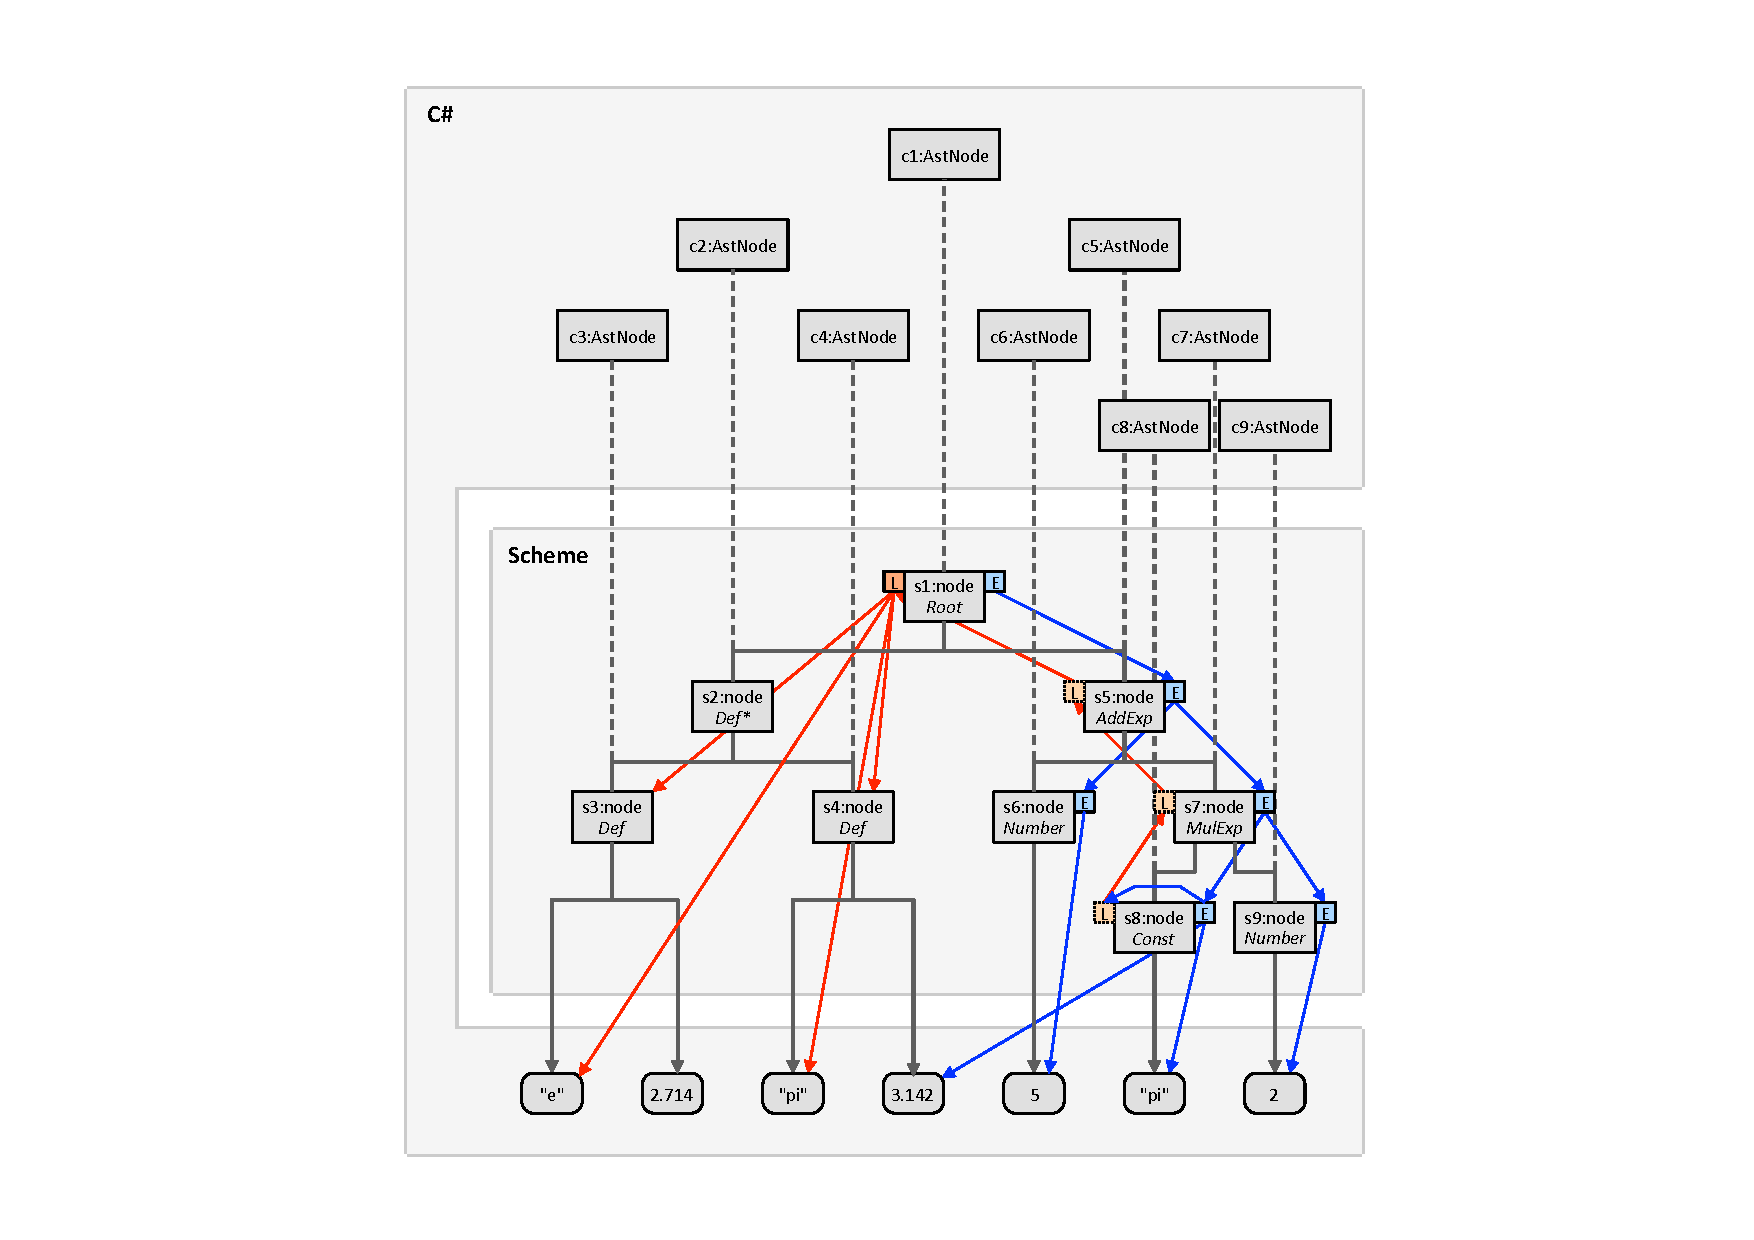
\includegraphics[width=0.9\linewidth]{figures/example-mapping.pdf}
	\caption{Beziehungen zwischen Adapter"=Objekten und \scm{node}"=Records im AST}
	\label{fig:bsp-graph}
\end{figure}

\section{Herausforderungen bei der Implementierung}\label{probleme}

Um das vorgestellte Verhalten der Schnittstelle zu realisieren, sind diverse programmiertechnische Hürden zu überwinden, die in diesem Kapitel nähergebracht werden sollen. Wichtig ist hierbei, dass die inkrementelle Auswertungssemantik RACRs für C\#"=Nutzer erhalten bleiben soll. Statt RACR in C\# nachzubauen, soll deshalb vielmehr die existierende Implementierung genutzt werden. Das impliziert, dass die RACR"=Scheme"=Implementierung alle AST- und Attributdaten hält und Zugriffe auf diese protokolliert, um einen dynamischen Abhängigkeitsgraphen zur inkrementellen Auswertung aufzubauen. Jeder Zugriff von C\# auf AST- und Attributdaten muss entsprechend auf RACR abgebildet werden. Andererseits sollen C\# Nutzer mit der Scheme"=Implementierung nicht in Berührung kommen, das heißt, nur mit nativen C\#"=Objekten arbeiten.

Um die Konsequenzen dieser Anforderungen bezüglich der Implementierung der Schnittstelle zu erläutern, soll auf das Anwendungsbeispiel aus Kapitel~\ref{anwendungsbeispiel} Bezug genommen werden. Abbildung~\ref{fig:bsp-graph} stellt die dort angelegten Objekte des ASTs und deren Beziehungen zueinander dar. Die schwarzen, durchgezogenen Linien und Pfeile repräsentieren die von RACR bei der AST"=Konstruktion erzeugen Assoziationen der \scm{node}"=Records zueinander beziehungsweise zu Terminalen.  Die bijektiven Assoziationen zwischen einer \csh{Racr.AstNode}"=Instanz und dem zugehörigen \scm{node}"=Record sind als gestrichelte Linien dargestellt. Die kleinen Quadrate repräsentieren die Attribute \scm{'Eval} (E) und \scm{'Lookup} (L). Die blauen beziehungsweise roten Pfeile kennzeichnen deren Abhängigkeiten auf weitere Attribute und Kind-Knoten. Der resultierende Graph wird von RACR zur inkrementellen Auswertung aufgebaut.

Entscheidend ist, dass \csh{Racr.AstNode}"=Instanzen keine Aggregationen zueinander besitzen. Sie fungieren lediglich als Proxy für die \scm{node}"=Objekte. Die eigentlichen Daten werden von RACR in Scheme gehalten. Jede AST- und Attributabfrage erfordert deshalb mehrfache Kontextwechsel zwischen C\# und Scheme. Während der Attributsauswertung registriert RACR diese Abfragen und baut zur Realisierung der inkrementellen Auswertung einen dynamischen Abhängigkeitsgraphen für das jeweilige Attribut auf.

\begin{figure}[]
	\centering
	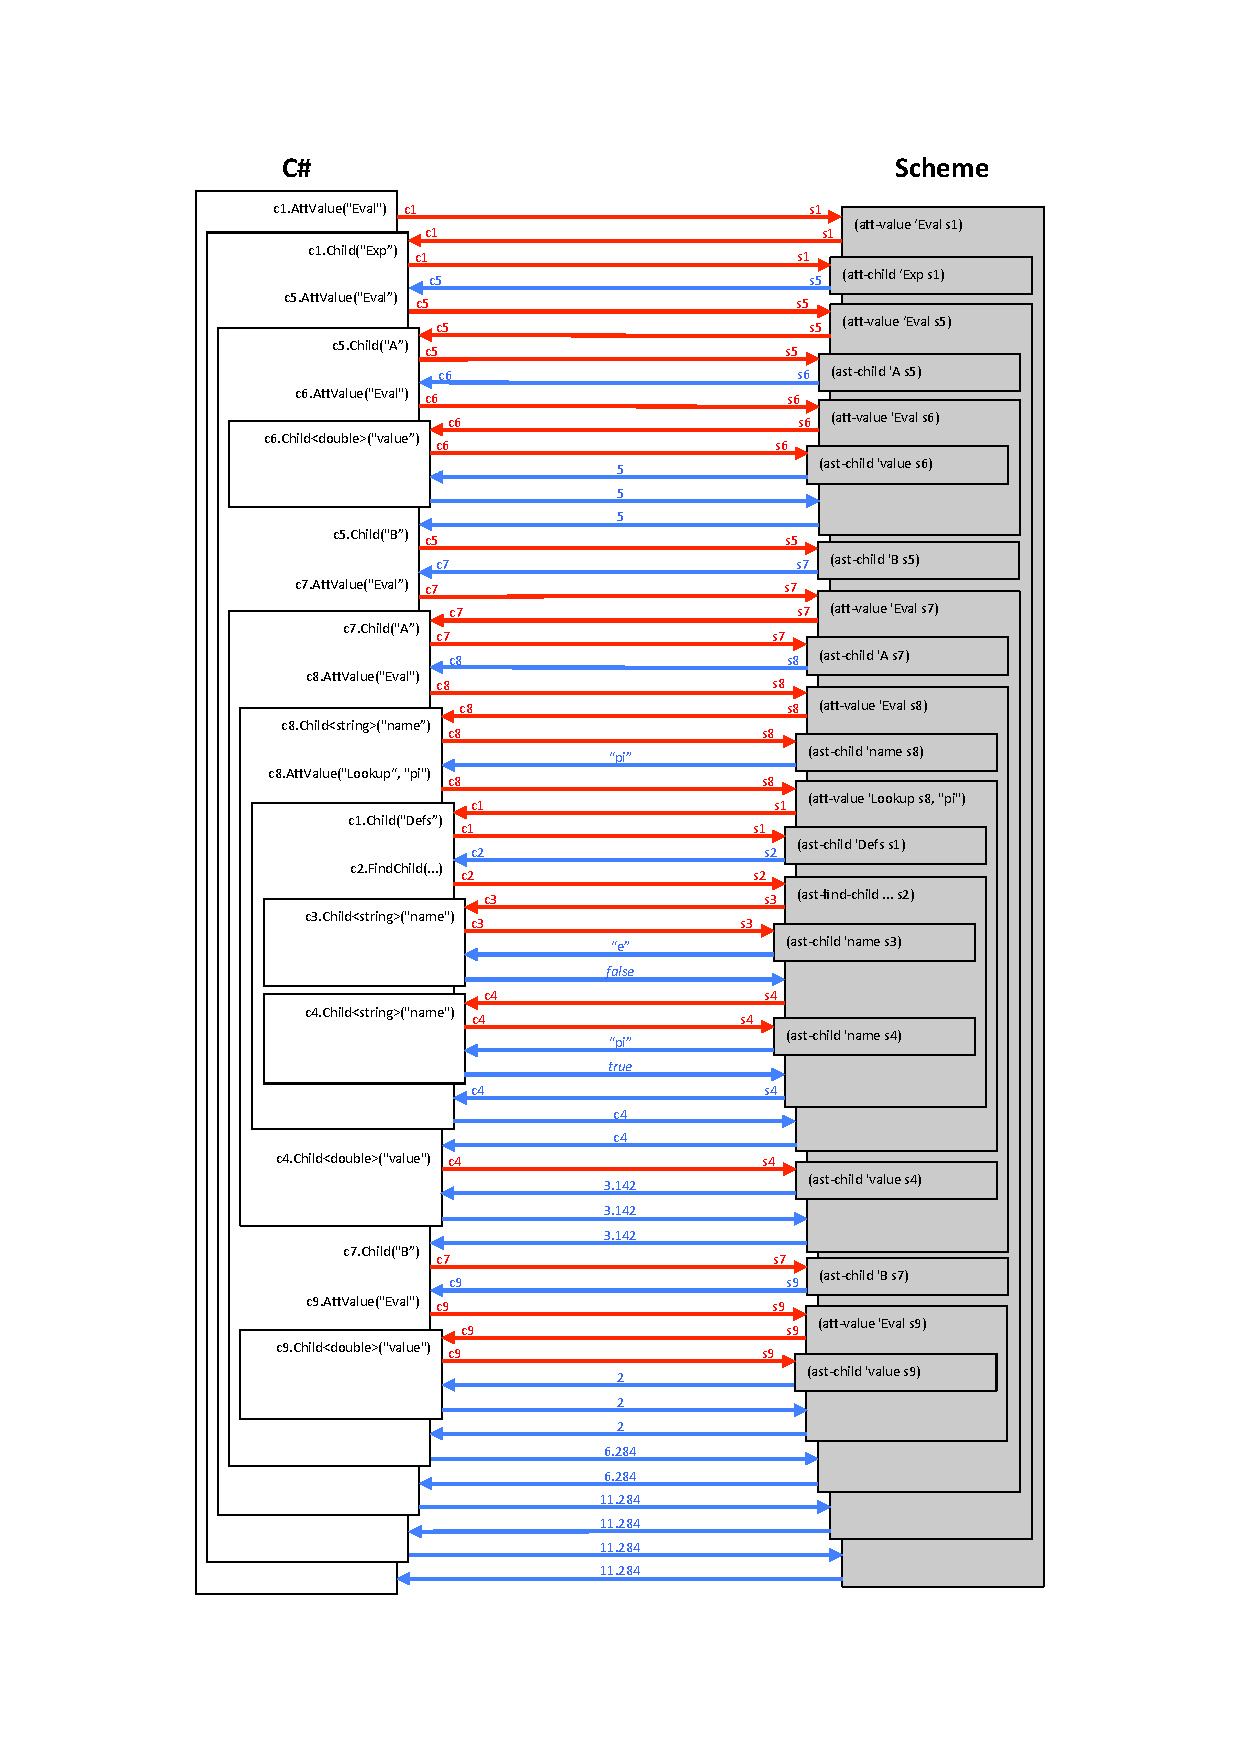
\includegraphics[scale=0.83]{figures/call-stack.pdf}
	\caption{Zeitliche Abfolge von API-Aufrufen}
	\label{fig:bsp-stack}
\end{figure}

Abbildung~\ref{fig:bsp-stack} veranschaulicht die zeitliche Abfolge von Methodenaufrufen der objektorientierten Schnittstelle (links) und parallel dazu die Aufrufe der Scheme-Prozeduren von RACR (rechts), die bei der Auswertung des Attributs \csh{"Eval"} auf dem Wurzelknoten ausgelöst werden. Rote Pfeile repräsentieren die Kontextwechsel bei Funktionsaufrufen. Für terminierende Funktionen sind die Kontextwechsel als blaue Pfeile dargestellt. Außerdem kennzeichnen Pfeile den Datenfluss von AST"=Knoten, wobei zwischen Nichtterminalen und Terminalen unterschieden wird. Für die Fälle, wo Nichtterminale übergeben werden, sind die Pfeile mit dem Namen der \csh{Racr.AstNode}"=Instanz und des \scm{node}"=Records aus Abbildung~\ref{fig:bsp-graph} beschriftet.

Der Aufruf von \csh{AttValue} auf der \csh{Racr.AstNode}"=Instanz \csh{c1} soll an RACR weitergeleitet werden, indem für den zugehörigen \scm{node}"=Record die Prozedur \scm{att-value} aufgerufen wird. Da die Attributcaches noch leer sind, muss die Attributgleichung für das Attribut \scm{'Eval} und dem Knotentyp \scm{'Root} ausgewertet werden. RACR ruft die zuvor via \scm{specify-attribute} angegebene Prozedur mit \scm{s1} als Argument auf. Diese Prozedur ist ein \csh{Callable}"=Objekt, in welchem das \csh{Delegate}"=Objekt von Quelltext~\ref{csh:bsp-attribute} (Zeile 2) gekapselt werden muss. Der Aufruf von \csh{Call} mit einem \scm{node}"=Record als Argument muss in dem Aufruf des Delegaten mit der entsprechenden \csh{Racr.AstNode}"=Instanz als Argument resultieren. Innerhalb des Delegaten wird auf \csh{c1} die Methode \csh{Child} aufgerufen, wo für den zugehörigen \csh{node}"=Record die Prozedur \scm{ast-child} aufgerufen wird. Diese gibt den Record \scm{s5} zurück. Der ursprüngliche \csh{Child}"=Aufruf muss diesen Record auf seine entsprechende \csh{Racr.AstNode}"=Instanz \csh{c5} abbilden. Es ist nicht hinreichend, wenn \csh{Child} einfach den \scm{node}"=Record zurückgäbe, da dies Anforderung \textbf{A5} verletzten würde. Die Wechsel zwischen C\# und Scheme setzt sich fort, bis der Ausdruck schließlich berechnet ist.

Es geht hervor, dass ein ständiger Kontextwechsel zwischen C\# und Scheme besteht. Zur Realisierung der Kontextwechsel von C\# zu Scheme bedarf es einer Abbildung von \csh{Racr.AstNode}"=Instanz auf \scm{node}"=Record. Das gleiche gilt entsprechend umgekehrt für Kontextwechsel von Scheme zu C\#. Methoden, die diese Abbildungen ausführen, müssen vorzugsweise leichtgewichtige Implementierungen haben, da sie notwendigerweise häufig aufgerufen werden. Im Wesentlichen ergeben sich also die drei folgenden Probleme:

\makeatletter
\let\orig@item\item

\def\item{%
	\@ifnextchar{[}%
	{\lstinline@item}%
		{\orig@item}%
}

\begingroup
\catcode`\]=\active
\gdef\lstinline@item[{%
\setbox0\hbox\bgroup
\catcode`\]=\active
\let]\lstinline@item@end
}
\endgroup

\def\lstinline@item@end{%
	\egroup
	\orig@item[\usebox0]%
}

\makeatother

\begin{description}
	\item[\textbf{Abbildung zwischen \csh{Racr.AstNode} und \scm{node}"=Record:}] Es muss die Möglichkeit geschaffen werden, zwischen der Scheme- und der C\#-Identität eines AST-Knotens zu wechseln. Diese Abbildung muss in allen Methoden, die auf \csh{Racr.AstNode}"=Instanzen arbeiten, zum Tragen kommen.
	\item[\textbf{Unterscheidung bei Kind-Knoten zwischen Terminalen und Nichtterminalen:}] In einigen Methoden, die uniform auf Terminalen wie Nichtterminalen angewendet werden, darf die besagte Abbildung nur bedingt eingesetzt werden, da in RACR Terminale als ungekapselte Wert"=Objekte gehandhabt werden.
	\item[\textbf{Wrapping der Attributsfunktionen:}] Der erste Parameter einer Attributsfunktion ist der AST"=Knoten, dessen Attribut ausgewertet werden soll. Aus der Sicht des C\#"=Nutzers handelt es sich um eine \csh{Racr.AstNode}"=Instanz. RACR übergibt zur Attributauswertung jedoch keine \csh{Racr.AstNode}"=Instanz, sondern den Handler des \scm{node}"=Records an das \scm{Callable}"=Objekt. Die Delegaten der Attributsgleichung müssen daher in einer Methode gekapselt werden, welche den \scm{node}"=Record auf dessen entsprechende \csh{Racr.AstNode}"=Instanz abbildet.
\end{description}

Die Lösung dieser Probleme ist Gegenstand des folgenden Kapitels.

\section{Implementierung}\label{implementierung}

In diesem Kapitel werden die Lösungen der in Kapitel~\ref{probleme} angeführten Probleme der Implementierung präsentiert.

\subsection{Brücke zwischen C\#- und Scheme-Objekten}\label{brücke}

Instanzen von \csh{Racr.Specification} und \csh{Racr.AstNode} müssen notwendigerweise den Handler des jeweiligen Scheme"=Records halten, um bei Methodenaufrufen diesen an die zugehörige Scheme"=Prozedur weiterleiten zu können. Im Konstruktor von \csh{Racr.Specification} wird via \csh{createSpecification.Call} ein neuer \scm{ast-spezifikation}"=Record angelegt, dessen Referenz in einem privaten Feld der Klasse, \csh{internal object} \csh{handler}, gespeichert wird. Alle weiteren Methoden leiten analog zum prozeduralen Ansatz die erhaltenen Daten an Aufrufe der zugehörigen \csh{Callable}"=Objekte weiter, jedoch unter der Benutzung von \csh{handler} als erstes Argument.

Gleichsam verhält es sich mit der Klasse \csh{Racr.AstNode}. Die Abbildung von einer \csh{Racr.AstNode}"=Instanz auf deren zugehörigen \scm{node}"=Record ist schlicht mit dem Zugriff auf \csh{handler} realisiert. Wie der Abbildung~\ref{fig:bsp-stack} zu entnehmen, ist jedoch eine unidirektionale Abbildung von \csh{Racr.AstNode}"=Instanzen auf \scm{node}"=Records nicht ausreichend. Eine Abbildung von \scm{node}"=Record auf \csh{Racr.AstNode}"=Instanz ist außerdem von Nöten. Dazu wird der Record um ein Feld ergänzt, das eine Referenz auf die Instanz hält.

\begin{lstlisting}[language=scm, caption={Angepasste Definition des \csh{node}"=Records}, label=scm:node]
(define-record-type node
  (fields
   (mutable evaluator-state)
   (mutable ast-rule)
   (mutable parent)
   (mutable children)
   (mutable attributes)
   (mutable cache-influences)
   (mutable annotations)
   (mutable csh-instance))      ; das neue Feld
  (opaque #t)(sealed #t)
  (protocol
   (lambda (new)
     (lambda (ast-rule parent children)
       (new #f ast-rule parent children
            (list) (list) (list)
            #f)))))             ; und dessen Initialwert
\end{lstlisting}

Quelltext~\ref{scm:node} zeigt die angepasste Definition des \scm{node}"=Records in \verb|racr/core.sls|. Auf Zeile~10 wird der Record um das Feld \scm{csh-instance} erweitert. Im Record-Konstruktor wird dieses vorerst auf \scm{#f} initialisiert. Des Weiteren müssen die Prozeduren zum Setzen (\scm{node-csh-instance-set!}) und Lesen (\scm{node-csh-instance}) des Felds aus der Scheme"=Bibliothek exportiert werden und im statischen Konstruktor von \csh{Racr} entsprechende \csh{Callable}"=Objekte initialisiert werden.

Nach der Erzeugung des \scm{node}"=Records im Konstruktor von \csh{Racr.AstNode} muss die \csh{this}"=Referenz in \scm{csh-instance} gespeichert werden. Die Hilfsfunktion \csh{GetNode} extrahiert die Referenz von dem Handler.

\begin{lstlisting}[language=csh]
private static AstNode GetNode(object ast) {
	return nodeCshInstance.Call(ast) as AstNode;
}
\end{lstlisting}

Mittels \csh{GetNode} und dem Zugriff auf \csh{handler} ist somit eine bidirektionale Abbildung zwischen \scm{node}"=Record und \csh{Racr.AstNode} geschaffen.

\subsection{Berücksichtigung von Terminalen}

Aufgrund der dynamischen Typisierung Schemes bietet RACR dem Nutzer eine generische Schnittstelle zum Zugriff auf Kinder- und Geschwister-Knoten – sowohl Terminale als auch Nichtterminale. In Kapitel~\ref{ast-knoten} wurde gezeigt, dass im Gegensatz dazu der Klasse \csh{Racr.AstNode} für den Zugriff auf Kind"= und Geschwister-Knoten für Terminale und Nichtterminale jeweils unterschiedliche Methoden bereitgestellt werden: Methoden für den Zugriff auf Terminale erwarten einen zusätzlichen Typ"=Parameter. Aus der Typsignatur einiger Methoden ist jedoch nicht ablesbar, ob es sich bei den übergebenen oder zu liefernden Knoten um Terminale oder Nichtterminale handelt. Nutzer müssen sich an die Grammatik der Spezifikation halten und die korrekten Akzessoren, mit gegebenenfalls passenden Typ"=Parameter, nutzen.

Auch in der Implementierung der Schnittstelle muss innerhalb dieser Methoden bei Kind-Knoten zwischen Nichtterminalen und Terminalen unterschieden werden können, um entsprechend die Abbildungsfunktionen einzusetzen beziehungsweise davon abzusehen, da die Abbildung nur bei Nichtterminalen zum Tragen kommen darf. Dies betrifft folgende Methoden von \csh{Racr.AstNode}: den Konstruktor, \csh{Children}, \csh{ForEachChild}, \csh{FindChild}, \csh{FindChildA}, \csh{RewriteRefine} und \csh{RewriteAbstract}. Diese Methoden realisieren die RACR"=Prozeduren \scm{ast-children}, \scm{ast-for-each-child}, \scm{ast-find-child}, \scm{ast-find-child*}, \scm{rewrite-refine} und \scm{rewrite-abstract}. RACR bietet eine Reihe undokumentierter Prozeduren zur Abfrage von Meta-Information bezüglich der AST-Schemas und Attribuierung für Spezifikationen eines ASTs. Folgende sind für den vorgestellten Zweck erforderlich:

\begin{itemize}
	\item \scm{(specification->find-ast-rule spec non-term)} liefert die einem Nichtterminal zugehörige AST"=Regel.
	\item \scm{(ast-rule->production rule)} liefert eine Liste mit den Produktionssymbolen einer AST"=Regel.
	\item \scm{(symbol->non-terminal? symbol)} bestimmt, ob ein Symbol ein Nichtterminal ist.
\end{itemize}

Die Objekte für AST"=Regeln und Symbole sind RACR"=interne Scheme"=Records. Mittels dieser Prozeduren wird im Konstruktor von \csh{Racr.AstNode} für jeden Kind"=Knoten bestimmt, ob er ein Nichtterminal ist. Diese Information wird aus Gründen der Effizienz direkt in der Klassen"=Instanz gespeichert, um gegebenenfalls wiederverwendet zu werden.

\begin{lstlisting}[language=csh, caption={Initialisierungen im Konstruktor von \csh{Racr.AstNode}}, label=csh:astnode-const]
public class AstNode {
	internal object handler;
	private bool[] ntChilren;
	public AstNode(Specification spec, string nonTerm,
				   params object[] children)
	{
		var nt = SymbolTable.StringToObject(nonTerm);
		var rule = specificationFindAstRule.Call(spec.handler, nt);
		var symbols = astRuleProduction.Call(rule) as Cons;
		ntChilren = new bool[children.Length];
		Cons list = null;
		Cons marker = null;
		for (int i = 0; i < children.Length; i++) {
			symbols = symbols.cdr as Cons;
			ntChilren[i] = symbolIsNonTerminal.Call<bool>(symbols.car);
			var child = ntChilren[i] ? (children[i] as AstNode).handler
									 : children[i];
			var cons = new Cons(child);
			if (list == null) list = marker = cons;
			else {
				marker.cdr = cons;
				marker = cons;
			}
		}
		handler = createAst.Call(spec.handler, nt, list);
		nodeCshInstanceSet.Call(handler, this);
	}
\end{lstlisting}

Quelltext~\ref{csh:astnode-const} zeigt diesen Vorgang. Der Konstruktor enthält eine \csh{for}"=Schleife, die das übergebene Kind"=Knoten"=Array traversiert. Parallel wird die Scheme"=Liste der Produktionssymbole durchwandert und die Information, ob ein Kind ein Nichtterminal ist, in \csh{ntChildren} gespeichert (Zeile~15). Zusätzlich wird eine Scheme"=Liste zur Weitergabe der Knote an \scm{create-ast} konstruiert: Für Nichtterminal"=Kinder wird aus der \csh{Racr.AstNode}"=Instanz der Handler auf den \scm{node}"=Record extrahiert (Zeile~16). Terminale werden direkt übergeben (Zeile~17). Interessant sind auch Zeilen~25 und 26, in denen \csh{handler} beziehungsweise \scm{csh-instance} gesetzt werden, wie in Kapitel~\ref{brücke} beschrieben.

In der Implementierung der übrigen, oben genannten Methoden, kann zur Unterscheidung von Terminalen und Nichtterminalen für den $n$-ten Kind-Knoten das entsprechende Element in \csh{ntChildren} konsultiert werden.

\subsection{Wrapping der Attributsfunktionen}

Attributsfunktionen werden in Form von Delegaten an die Methode \csh{SpecifyAttribute} der Klasse \csh{Racr.Specification} übergeben. Quelltext~\ref{csh:falsche-specattr} zeigt eine naive Implementierung, in welcher analog zur Implementierung der prozeduralen Schnittstelle auf dem \csh{Delegate}"=Objekt IronSchemes die Extension-Methode \csh{ToSchemeProcedure} aufgerufen wird um ein \csh{Callable}"=Objekt zu erzeugen, das anschließend an den Aufruf der Scheme"=Prozedur \scm{specify-attribute} übergeben wird.

\begin{lstlisting}[language=csh, caption={Naive Implementierung von \csh{SpecifyAttribute}}, label=csh:falsche-specattr]
public void SpecifyAttribute(string name, string nonTerm, string context,
							 bool cached, Delegate equation)
{
	specifyAttribute.Call(
		handler,
		SymbolTable.StringToObject(name),
		SymbolTable.StringToObject(nonTerm),
		SymbolTable.StringToObject(context),
		cached,
		equation.ToSchemeProzedure(),
		false);
}
\end{lstlisting}

Wie in Kapitel~\ref{spezifikation} vorgestellt, soll der erste Parameter einer Attributsfunktion vom Typ \csh{Racr.AstNode} sein. Der Attributauswerter RACRs (die Prozedur \scm{att-value}) erwartet jedoch Attributsfunktionen, deren erstes Argument ein RACR \scm{node}"=Record ist — der AST Knoten mit welchem die auszuwertende Attributsinstanz assoziiert ist. Die Auswertung einer in C\# definierten Attributsfunktionn löst demnach einen Laufzeitfehler aus, da innerhalb des \csh{Callable} der Versuch, den \scm{node}"=Record des AST-Knoten in eine \csh{Racr.AstNode}"=Instanz umzuwandeln scheitert. Auf dem \csh{Delegate}"=Objekt, das die Attributsgeichung hält, kann \csh{ToSchemeProcedure} zur Erzeugung eines \csh{Callable}"=Objekts nicht direkt angewandt werden. Die Delegaten müssen in einer weiteren Methode gekapselt werden, innerhalb welcher die Abbildung von \scm{node}"=Record auf \csh{Racr.AstNode}"=Instanz zum Einsatz kommen muss. Analog zur prozeduralen Schnittstelle, müssen beliebig typisierte Rückgabewerte sowie etwaige weitere Parameter unterstützt werden (siehe Kapitel~\ref{prozeduren}). Da die Typsignatur des Delegaten während der Übersetzung unbekannt ist, muss mithilfe von Reflexion eine passende Wrapper"=Methode zur Laufzeit generiert werden.

Wegen der dynamischen Typisierung Schemes sind Parameter und Rückgabewert der Methode \csh{Call} der \csh{Callable}"=Schnittstelle allesamt mit \csh{object} typisiert. Für Delegaten, die von Scheme aus aufgerufen werden sollen, sich jedoch in der Typsignatur von \csh{Call} unterscheiden, wird in der Methode \csh{ToSchemeProcedure} eine Wrapper"=Methode erzeugt, in welcher entsprechende Typumwandlungen ausgeführt werden. Für mit einem Werttypen typisierte Parameter des Delegaten muss eine Konvertierung von \csh{object} zu diesem Werttypen realisiert werden (Unboxing). Ähnlich verhält es sich mit den Rückgabewerten, wobei gegebenenfalls von Werttyp nach \csh{object} konvertiert wird (Boxing). Derartige Typumwandlungen sind rechentechnisch aufwendig. Ein doppeltes Methoden-Wrapping ist daher zu vermeiden. Es soll eine dynamische Methode erzeugt werden, in welcher einerseits die Abbildungsfunktion auf den AST"=Knoten, also den ersten Parameter des Delegaten, angewendet wird und zusätzlich für alle übrigen Parameter und den Rückgabewert das Unboxing beziehungsweise Boxing ausgeführt wird, unter der Bedingung, dass es sich jeweils um einen Werttypen handeln.

C\# umfasst eine Schnittstelle, um zur Laufzeit dynamische Methoden zu erzeugen. Damit in Verbindung bietet IronScheme die leichtgewichtige Fabrikmethode \csh{Closure.Create}, welche ein \csh{Delegate}"=Objekt erwartet, dessen Parameter und Rückgabewert mit \csh{object} typisiert sind, und ein \csh{Callable} liefert. Dieses Objekt hält im Wesentlichen eine Referenz auf den Delegaten. Der entscheidende Unterschied von \csh{Closure.Create} zu \csh{ToSchemeProcedure} besteht darin, dass dabei kein Wrapping des \csh{Delegate} (Unboxing und Boxing) ausgeführt werden muss, da die Signatur des Delegaten bereits in der notwendigen Form vorliegt.

\begin{lstlisting}[language=csh, caption={Dynamische Methodengenerierung und Typzuordnung}, label=csh:wraptocallable]
static Callable WrapToCallable(this Delegate equation) {
	MethodInfo method = equation.Method;
	Type[] paramTypes = method.GetParameters()
	.Select(p => p.ParameterType).ToArray();
	if (paramTypes.Length == 0
	|| !typeof(AstNode).IsAssignableFrom(paramTypes[0])) {
		throw new ArgumentException(
				"type of delegate's first argument must be AstNode.");
	}

	var dynmeth = new DynamicMethod("", typeof(object),
						paramTypesArray[paramTypes.Length], true);
	var gen = dynmeth.GetILGenerator();

	gen.Emit(OpCodes.Ldarg_0);
	var getNodeInfo = ((Delegate)(Func<object, AstNode>)GetNode).Method;
	gen.Emit(OpCodes.Call, getNodeInfo);
	
	for (int i = 1; i < paramTypes.Length; i++) {
		gen.Emit(OpCodes.Ldarg_S, i);
		if (paramTypes[i].IsValueType) {
			gen.Emit(OpCodes.Unbox_Any, paramTypes[i]);
		}
		else {
			gen.Emit(OpCodes.Castclass, paramTypes[i]);
		}
	}
	gen.Emit(OpCodes.Call, method);
	if (method.ReturnType.IsValueType) {
		gen.Emit(OpCodes.Box, method.ReturnType);
	}
	gen.Emit(OpCodes.Ret);

	Type outType = callTargets[paramTypes.Length];
	return Closure.Create(dynmeth.CreateDelegate(outType),
						  paramTypes.Length);
}
\end{lstlisting}

Quelltext~\ref{csh:wraptocallable} zeigt die Implementierung der statischen Methode \csh{WrapToCallable}, welche \csh{ToSchemeProzedure} in Quelltext~\ref{csh:falsche-specattr} (Zeile~10) ersetzen soll. Der wichtigste Teil der Methode umfasst die Zeilen~15 bis 32. Hier wird der IL"=Code der dynamischen Methode festgelegt. Dabei werden Opcodes für das Laden von Argumenten, Methodenaufrufe, Unboxing und Boxing, sowie das Beenden der Methode eingesetzt. Folgende Schritte sollen in der zu erzeugenden Wrapper"=Methode ausgeführt werden: Zuerst wird der erste Parameter (der AST-Knoten) geladen und anschließend \csh{GetNode} aufgerufen (Zeile~15 bis 17). Als nächstes werden alle weiteren Parameter geladen (Zeile~20). Falls es sich bei deren Typ um Werttypen handelt, wird Unboxing ausgeführt (Zeile~22). Für Referenztypen muss stattdessen eine dynamische Typumwandlung erfolgen (Zeile~25). Schließlich wird das \csh{Delegat}"=Objekt aufgerufen, innerhalb welchem der Attributwert berechnet werden soll (Zeile~28). Wenn der Attributwert mit einem Werttyp typisiert ist, so wird Boxing angewendet (Zeile~29 bis 31). Damit terminiert die dynamische Methode (Zeile~32).

Nun wird aus dem \csh{DynamicMethod}"=Objekt mittels \csh{CreateDelegate} ein \csh{Delegat} erzeugt, das anschießend an \csh{Closure.Create} übergeben wird (Zeile~32 und 33). Das resultierende \csh{Callable} ist eine Attributsfunktion, welche einerseits in C\# definiert wurde (und daher nur unter Beachtung der objektorientierten Schnittstelle von RACR-NET implementiert wurde) und andererseits vom Attributsauswerter der existierenden RACR"-Scheme"-Implementierung verarbeitet werden kann. Somit ist das generierte \csh{Callable} eine korrekte C\#"=Attributsfunktion für \scm{specify-attribute}.

	% This program and the accompanying materials are made available under the
% terms of the MIT license (X11 license) which accompanies this distribution.

% Author: D. Langner, C. Bürger

\chapter{Evaluation}\label{eval}

Es wurde bereits an dem Anwendungsbeispiel in Kapitel~\ref{anwendungsbeispiel} gezeigt, dass die an die RACR-NET Schnittstelle gesetzten funktionalen Anforderungen von der vorgestellten Implementierung erfüllt werden, insbesondere bezüglich einer benutzerfreundlichen objektorientierten Schnittstelle. Der Zugriff auf Spezifikation und AST-Knoten erfolgt ausschließlich über Instanzen von \csh{Racr.Specification} beziehungsweise \csh{Racr.AstNode} und alle Aufrufe von RACR sind in Methoden dieser Stellvertreter"=Objekte gekapselt.

Im Folgenden soll gezeigt werden, dass RACR-NET nicht nur benutzerfreundlich, sondern auch korrekt und effizient ist.

\section{Testen der Schnittstelle}

Zum Testen von RACR-NET wurde eine umfangreiche, bereits existierende Anwendung\footnote{\url{https://github.com/christoff-buerger/racr/tree/master/examples/questionnaires}}, die den wesentlichen Funktionsumfang RACRs abdeckt, in C\# reimplementiert. Das Beispiel ist eine Lösung des Language Workbench Challenge 2013~\cite{Erdweg2013}, dessen Aufgabe\footnote{\url{http://www.languageworkbenches.net/wp-content/uploads/2013/11/Ql.pdf}} darin bestand, eine domänenspezifische Sprache zu schaffen, mittels welcher interaktive Fragebögen zur Datenerfassung auf einfache Weise beschrieben und ausgewertet werden können. Die Anwendung bedient sich aller Mechanismen RACRs mit Ausnahme von komplexeren Graphersetzungen. Um auch die funktionelle Korrektheit der Graphersetzungsmethoden sicherzustellen, wurden diese in einem eigenen NUnit\footnote{\url{http://www.nunit.org/}}-Test erfasst.

\section{Performance-Messungen und -Vergleiche}

Die Erzeugung von Adapter"=Objekten und der indirekte Zugriff auf RACRs Funktionalitäten über jene Objekte erzeugt einen Laufzeit-Overhead. Dieser wurde für eine RACR"=Anwendung ermittelt, die im Folgenden beschrieben wird.

Unter Verwendung der in Kapitel~\ref{anwendungsbeispiel} gegebenen Sprachspezifikation wurden arithmetische Ausdrücke für verschiedene Konstantenbelegungen berechnet. Um die Ausführungszeiten des C\#-Programms gegenüber denen des Scheme-Programms vergleichen zu können, wurde die Anwendung in beiden Sprachen, Scheme (unter der Verwendung der RACR Scheme-Bibliothek) und C\# (mittels der objektorientierten Schnittstelle), implementiert. Der Laufzeit"=Overhead ist die Differenz der Ausführungszeiten beider Implementierungen in IronScheme. Die den zu berechnenden Ausdruck repräsentierenden ASTs wurden mithilfe eines Python-Skripts generiert und enthalten jeweils 5.000, 10.000 und 20.000 Binär-Operationen und ebenso viele Blatt-Knoten. Die Hälfte der Blatt-Knoten sind Konstanten, wobei insgesamt 26 verschiedene Konstanten-Definitionen benutzt werden.

\begin{table}[h!]
	\centering
	\begin{tabu} to 0.8\textwidth { X[r] X[r] X[r] X[r] X[r] X[r] }
		\toprule
			&&& \multicolumn{3}{c}{Laufzeit in s} \\ \cmidrule(r){4-6}
			Operationen & Evals & Rewrites & C\# & IronScheme & Racket \\
		\midrule
			 5.000 &     1 &     0 &   1,43 &   1,36 &   0,45 \\
			10.000 &     1 &     0 &   2,93 &   2,92 &   0,98 \\
			20.000 &     1 &     0 &   6,21 &   6,03 &   2,17 \\
%			40.000 &     1 &     0 &  12,76 &  12.34 &   4,55 \\
			 5.000 & 1.000 & 1.000 &  72,44 &  72,20 &  24,31 \\
			10.000 & 1.000 & 1.000 & 150,14 & 145,81 &  71,08 \\
			20.000 & 1.000 & 1.000 & 330,58 & 316,97 & 217,79 \\
%			40.000 & 1.000 & 1.000 & 704,30 & 690.11 & 582.17 \\
		\bottomrule
		\end{tabu}
	\caption{Performance-Messungen}
	\label{measurements}
\end{table}

Alle Läufe wurden auf einem Rechner mit einem Intel Core i5-3350P Vier-Kern-Prozessor und 16~GB RAM unter Windows~8.1 gemessen. Das verwendete IronScheme Release war 115404, 32-Bit, vom 29. Oktober 2015. Als .NET VM wurde das Microsoft .NET Framework 4.0 verwendet. Von zwanzig Messungen pro Lauf wurde die beste Zeit genommen. Tabelle~\ref{measurements} zeigt die Messergebnisse für eine einzelne Berechnung des Attributs \scm{'Eval} (Zeile~1 bis 3). Ferner wurden innerhalb einer Schleife jeweils der Wert einer Konstanten in deren Definition modifiziert und anschließend \scm{'Eval} für den Wurzel-Knoten ausgewertet (Zeile~4 bis 6).

Um die Performance von IronScheme gegenüber anderen Scheme-VMs abschätzen zu können, wurden die Tests ebenfalls auf der Racket\footnote{\url{http://racket-lang.org/}} Scheme-VM durchgeführt (Racket Version 6.2). Zur Erfassung des durch die objektorientierte Schnittstelle generierten Overheads sind jedoch lediglich die für IronScheme gemessenen Ausführungszeiten relevant.

Die Messungen ergeben, dass die RACR-NET-Lösung erwartungsgemäß etwas langsamer ausführt als eine reine Scheme"=Lösung. Der Performance-Overhead beträgt für 20.000 Knoten und 1.000 Auswertungen und Graphersetzungen circa 4,3\,\% und ist damit durchaus akzeptabel. Des Weiteren wird ersichtlich, dass IronScheme zwar langsamer ist als Racket, der Faktor jedoch keine Größenordnung beträgt (Im Gegensatz zu Racket ist IronScheme ein Ein-Man-Projekt, bei dem Performance nicht im Mittelpunkt steht).

Bei dem gewählten Beispiel handelt es sich um eine Referenzattributgrammatik, deren Attributsgleichungen auf simple Addition und Multiplikation zweier Fließkommazahlen beschränkt sind. Es bleibt daher zu untersuchen, wie stark der Geschwindigkeitsvorteil von C\# gegenüber IronScheme in komplexeren Gleichungen zum Tragen kommt und, ob dieser den Overhead von RACR-NET wohl möglich kompensiert.

Die Messergebnisse unterstreichen die Vorteile der RAG-gesteuerten Graphersetzung. Eine einmalige Auswertung von \scm{'Eval} ist relativ teuer (1,43 Sekunden mittels RACR-NET), weil anfangs alle Attribut-Caches leer sind und so \scm{'Eval} erst für jeden Teilausdruck berechnet werden muss. Da die vorgenommenen Graphersetzungen nur jeweils einen Anteil der zuvor berechneten Attributwerte invalidieren, begünstigt die inkrementelle Auswertung alle nachträglichen Berechnungen. Eintausend Berechnungen mit intermediären Graphersetzungen benötigen 330,58 Sekunden – nur circa 20\,\% der tausendfachen Dauer der initiale Berechnung.

	% This program and the accompanying materials are made available under the
% terms of the MIT license (X11 license) which accompanies this distribution.

% Author: D. Langner, C. Bürger

\chapter{Zusammenfassung und Ausblick}\label{ausblick}

Abschließend wird der Beitrag dieser Arbeit noch einmal zusammengefasst und ein Ausblick auf offene Fragen und Erweiterungsmöglichkeiten gegeben.

\section{Eine objektorientierte Bibliothek für RAG-gesteuerte Graphersetzung}

In dieser Arbeit wurde die Umsetzung einer objektorientierten Schnittstelle von RACR, der Scheme"=Bibliothek zur Referenzattributgrammatik"=gesteuerten Graphersetzung, für die Software"=Plattform .NET präsentiert. Diese Schnittstelle namens RACR"=NET ermöglicht es, RACR"=Anwendungen in C\# zu programmieren.

IronScheme, eine Scheme-Implementierung für .NET, wurde als virtuelle Maschine eingesetzt, um innerhalb der Methoden der Schnittstelle die entsprechenden RACR-Prozeduren aufzurufen. Da sich IronScheme zur Ausführung von RACR-Anwendungen als nicht hinreichend R6RS-konform herausstellte, wurden geringfügige Veränderungen am Quellcode RACRs bezüglich der \scm{hashtable}"=Prozeduren vorgenommen, um Grenzfälle zu umgehen. Unter Verwendung der IronScheme"=Klassenbibliothek wurde erst eine imperative Schnittstelle geschaffen. Darauf aufbauend entstand eine benutzerfreundliche, objektorientierte Schnittstelle, die den vollständigen Funktionsumfang RACRs über Stellvertreter"=Objekte für Spezifikationen und AST"=Knoten abbildet.

In der Schnittstelle kommen keine Scheme-spezifischen Datentypen zum Einsatz, sodass Nutzer RACR"=NET ohne jegliche Scheme"=Kenntnisse einsetzen können. Gleichzeitig bleibt die Nähe zu RACRs originalen Scheme"=Schnittstelle bewahrt. Der indirekte Zugriff auf AST"=Knoten erzeugt in RACR-NET"=Anwendungen einen Performance"=Overhead gegenüber äquivalenten, via IronScheme ausgeführten RACR"=Anwendungen. Dieser wurde für eine Beispiel"=Anwendung bestimmt und beträgt 4,3\,\%.

\section{Zukünftige Arbeiten}

RACR-NET dient dem Zweck, die RAG"=gesteuerte Graphersetzung von dem gewählten Technikraum .NET aus nutzen zu können. Bisher wurde nur gezeigt, wie die Schnittstelle von C\# aus eingesetzt wird. Es existiert jedoch eine Vielzahl von .NET"=Sprachen, innerhalb welcher RACR-NET eingesetzt werden kann. Inwieweit dies für solche Sprachen effektiv umgesetzt werden kann, die neben Objektorientierung andere Programmierparadigmen verfolgen (zum Beispiel F\# mit der funktionale Programmierung), muss noch untersucht werden.

Ein interessanter Anwendungsfall besteht darin, bereits bestehende in Scheme implementierte RACR"=Anwendungen von C\# aus über RACR-NET zu erweitern. Dies schließt die Möglichkeit ein, AST"=Schemas um zusätzliche AST"=Regeln zu ergänzen und weitere Attribute zu definieren. Um die Erweiterbarkeit einer via Scheme spezifizierten Sprache in C\# zu ermöglichen und Kopplung und Vererbung von Attributgrammatiken über Sprachgrenzen hinaus zu realisieren, bedarf es weiterer Arbeit. Eine wichtige Aufgabe liegt dabei in der Sonderbehandlung des Falls, dass in Scheme definierte Referenzattribute in C\# ausgewertet werden, da diese als AST"=Knoten statt eines Stellvertreter"=Objekts ein RACR"=internes Objekt liefern. Der korrekte Umgang mit diesen Datentypen setzt Scheme"=Kenntnisse voraus, die RACR-NET in den jetzigen Anwendungsszenarien nicht verlangt.

	\part*{Anhänge}
	\appendix
	\chapter{Literaturverzeichnis}
	\printbibliography[heading=none]
	\chapter{MIT Lizenz}
	\input{../../license.txt}
\end{document}
